% vim: nospell
% mainfile: master.tex
\input set/preamble.tex
\input set/macros.tex
\input set/listings.tex

\begin{document}

% Front matter %%%%%%%%%%%%%%%%%%%%%%%%%%%%%%%%%%%%%%%%%%%%%%%%%%%%%%%%%%%%%%%%%
\pagenumbering{roman}
\pagestyle{empty}
\input set/frontpage
\input set/titlepage
\pagestyle{fancy}
\setcounter{page}{1}
\tableofcontents
\cleardoublepage

% Main matter %%%%%%%%%%%%%%%%%%%%%%%%%%%%%%%%%%%%%%%%%%%%%%%%%%%%%%%%%%%%%%%%%%
\setcounter{page}{1}
\pagenumbering{arabic}

% Intro
\chapter{Introduction}
\label{cha:intro}
Smartphones and the need for high data rates have become an integrated part of the our everyday lives. The focus on data rates have become apparent with the standardization fo the 4th Generation (4G) of mobile communications, featuring Long Term Evolution (LTE) and LTE-Advanced (LTE-A) which both are to increase the data throughput. 

The specifications of 4G increase the number of antennas (MIMO), extend the bandwidth and define Carrier Aggregation (CA) combinations, among others. The operating frequencies for 4G are scattered around, ranging from \SIrange{698}{2690}{MHz}. Developing small handset antennas that can cover all these bands is a challenge for the antenna engineers, particularly for the lower bands, due to the fundamental limits and trade-offs between size, bandwidth and efficiency\cite{}. However the lower bands offer attractive features such as high building penetration and wide range cell-coverage. 

One way to overcome this problem is by using frequency-reconfigurability, to achieve good efficiency in the low bands and increase the number of bands that can be covered. Tuning can be performed on the antenna feeding line \cite{} \cite{} or on the antenna element \cite{} \cite{}. In this project MEMS tunable capacitors are used, since they offer low insertion loss, high voltage handling, and low power consumption\cite{}. Furthermore, the project aims to develop tunable antennas supporting MIMO operation on LTE bands for a handset. 
\fixme{Update cites}

\section{Reading Guidelines}
Throughout the report, a lot of sweep-plots will be presented with many plots per figure. The color order presented in Figure~\ref{fig:colororder} is used for all sweeps so the first plot is always blue, the next is green, and so forth.

\definecolor{bb}{rgb}{0.0, 0.0, 1.0}
\definecolor{gg}{rgb}{0.0, 0.5, 0.0}
\definecolor{rr}{rgb}{1.0, 0.0, 0.0}
\definecolor{cc}{rgb}{0.0, 0.75, 0.75}
\definecolor{mm}{rgb}{0.75, 0.0, 0.75}
\definecolor{yy}{rgb}{0.75, 0.75, 0.0}
\definecolor{kk}{rgb}{0.0, 0.0, 0.0}
\begin{figure}[htbp]
    \centering
    \begin{tikzpicture}[scale=0.5]
        \foreach \x/\c in {1/bb, 2/gg, 3/rr, 4/cc, 5/mm, 6/yy, 7/kk} {
            \fill[\c] (\x, 0) rectangle ++(1,1);
            \path (\x,1) ++ (right:0.5) node[above] {\x};
        };
    \end{tikzpicture}
    \caption{Color order for sweep plots in the report.}
    \label{fig:colororder}
\end{figure}

When two-port S-parameter measurements are mentioned in the report, port 1 is always the top-antenna and port 2 is the side-antenna unless otherwise noted.


\section{Initiating Problem}
\label{sec:init_problem}


% Analysis
\chapter{Post Processing}
\label{cha:postproc}

In this chapter, the libraries for post processing data from CST and Satimo will be described. The libraries are written in Python. By the end of the chapter, usage examples will be given.

\section{Data Format}
The trx files, from Satimo Passive Measurement, contain data formatted in four columns:
\begin{enumerate}
    \item Horizontal polarization, real part.
    \item Horizontal polarization, imaginary part.
    \item Vertical polarization, real part.
    \item Vertical polarization, imaginary part.
\end{enumerate}
Each column contains 
\begin{equation}
    n_r =  n_f \times n_a \times n_e
\end{equation}
where
\begin{where}
\item[$n_r$] Total number of rows per column.
\item[$n_f$] Number of different frequencies in the measurement.
\item[$n_a$] Number of azimuth coordinates (usually 8).
\item[$n_e$] Number of elevation coordinates (usually 15).
\end{where}
The first $n_a \times n_e$ rows are for the first frequency and the next $n_a \times n_e$ rows are for the second frequency. Within this, the first $n_e$ rows are for the first azimuth angle and so on.

To get a better overview, the basic format for the following libraries is a $\theta \times \phi$-matrix like the following:
\begin{equation}
    M = \begin{bmatrix}
        m_{1,1} & m_{1,2} & \dots & m_{1,n} \\
        m_{2,1} & m_{2,2} & \dots & m_{2,n} \\
        \vdots & \vdots & & \vdots \\
        m_{m,1} & m_{m,2} & \dots & m_{m,n}
    \end{bmatrix}
\end{equation}
The data is rearranged to have $\phi$ go from \ang{0} to \ang{360} and $\theta$ from \ang{0} to \ang{180} as shown in Table~\ref{tab:matrixformat}.

\begin{table}[htbp]
    \centering
    \begin{tabular}{|l|c|c|}
        \hline
        Elements & $\theta$ & $\phi$ \\
        \hline
        $m_{1,1}$ & \ang{0} & \ang{0} \\
        $m_{1,n}$ & \ang{0} & $\ang{360}$ \\
        $m_{m,1}$ & \ang{180}$^{\dagger}$ & \ang{0} \\
        \hline
    \end{tabular}
    \caption{Format of $\theta\times\phi$-matrix. $^{\dagger}$For Satimo measurements, this is $180-22.5=\ang{157.5}$ because of the blind spot in the bottom.}
    \label{tab:matrixformat}
\end{table}

\section{Basic Antenna Parameters}
This section will give a summery of the fundamental theories and parameters that are used to describe antennas. This should give a basic understanding of antennas and the parameters described in this section are used throughout the report. 

\subsection{Antenna Definition}
\label{subsec:antenna-def}
The IEEE defines an antenna as: ``a means for radiating or receiving radio waves''. In other words, the purpose of an antenna is to make the transistion from a signal in a transmission line to electromagnetic fields in the air. An antenna will radiates an electric field (E-field) in a given direction, which then induces a magnetic field (H-field) orthogonal to the E-field, this relation is described by Maxwell's Equations which is covered in Section~\ref{sec:fdtd}. \cite{}

\subsection{Isotropic Radiator}
\label{subsec:isotropic-ant}
An isotropic antenna, can be represented as a point source. The isotropic antenna radiates its power uniformly in a sphere. The power density $S_{iso}$ can be expressed as the source power $P_s$ over the surface area of a sphere which is given by $4\pi r^2$. \cite{} 

\begin{align}
  S_{iso} = \frac{P_s}{4\pi r^2}
\end{align}

Clearly it is not possible to construct such an antenna, however it is used as a reference for quantifying other properties of the antenna. These properties could be the gain or directivity (See Section\ref{subsec:dir_gain}), and the unit would then be in \si{dBi} rather than \si{dB}.

\subsection{Radiation Pattern}
\label{subsec:radiation-p}
The radiation pattern describes how the antenna emits or receives radiated power. This is commonly visualized by a 3D plot or 2D cuts of the 3D plot in specific coordinates. The unit of power used is often gain or directivity (See Section~\ref{subsec:dir_gain}) and this is often compared to the isotropic antenna. \cite{}

\subsection{Field Regions}
The waves transmitted from the antenna are usually grouped into three regions of radiation, based on how the waves propagate and the field structure\cite{balanis2012antenna}. Obviously there is no abrupt change, but rather a continuous change.

\begin{itemize}
\item The Reactive near-field 
\item The Radiating near-field (Fresnel)
\item The Far-field
\end{itemize}

The reactive near-field is defined as the portion of the near-field region immediately surrounding the antenna wherein the reactive field predominates\cite{balanis2012antenna}. The outer boundary for this region is given by $R < 0.62 \sqrt{\frac{D^3}{\lambda}}$\cite{balanis2012antenna}.

The radiating near-field is defined as the region between the reactive near-field and the far-field, this field might not exist in the case that the overall antenna dimension is very small compared to the wavelength. The outer boundary for this is defined as $R \geq \frac{2D^2}{\lambda}$\cite{balanis2012antenna}.

The far-field region is defined as the region of the field where the angular field distribution is independent of the distance, that is the radiation pattern does not change shape with distance. The far-field is also dominated by fields where the E- and H-fields are orthogonal and propagates as plane waves. The inner boundary is given as $R = \frac{2D^2}{\lambda}$\cite{balanis2012antenna}.

These different regions are illustrated on Figure~\ref{fig:field-regions}. 

\begin{figure}[htbp]
  \centering
  \includegraphics[scale=1]{img/analysis/radiationfields}
  \caption{Visualization of different fields \cite{balanis2012antenna}.}
  \label{fig:field-regions}
\end{figure}

\subsection{Directivity and Gain}
\label{subsec:dir_gain}
Directivity is defined as the ratio of the power radiated at a  point with a certain angle and distance from the antenna compared to what would be radiated from a reference isotropic antenna. Mathematically it can be written as \cite{}: 
\begin{align}
  D = \frac{U}{U_0} = \frac{4 \pi U}{P_{rad}} 
\end{align}
where
\begin{where}
  \item[$D$] is the directivity
  \item[$U$] is the radiation intensity
  \item[$U_0$] is the radiation intensity of an isotropic source
  \item[$P_{rad}$] is the total radiated power 
\end{where}
It should be noted, that for this equation to be valid, the waves must propagate as plane waves, thus being in the far-field region.


Gain is a measure closely related to directivity, it takes the antenna efficiency of the antenna into account as well as the direction. The gain is defined as the ratio of the intensity in a given direction to the radiant intensity that would be obtained if it was radiated isotropically. In mathematical form it can be expressed as \cite{}:

\begin{align}
  G = 4 \pi \frac{\text{radiation intensity}}{\text{total accepted input power}} = 4 \pi \frac{U(\theta,\phi)}{P_{in}}
\end{align}

In many cases the relative gain is used, which is defined as the ratio of the power gain in a given direction to the power gain of a reference antenna in its referenced direction. The reference antenna could be a dipole, horn etc. 

The gain can also be calculated using the directivity, since they are only related by the efficiency. This is given as: \cite{}

\begin{align}
  G(\theta,\phi) = e_{cd}D(\theta, \phi) 
\end{align}

\subsection{Impedance, Return Loss and VSWR}
The impedance and matching is an important part of the antenna design to ensure maximum power transfer. The input impedance of an antenna is defined as $Z_{\text{in}}$. From the classical circuit theory it is known that the maximum power transfer occurs when the in- and output impedance is matched. If there is a mismatch some of the power will be reflected back into the source, and thus not transmitted from the antenna. The reflection coefficient $\Gamma$ is defined as: \cite{}

\begin{align}
  \Gamma = \frac{Z_{in}-Z_0}{Z_{in}+Z_0} 
\end{align}
where
\begin{where}
\item[$Z_0$] denotes the characteristic impedance, which is classically \SI{50}{\ohm}
\end{where}
The reflection coefficient is furthermore often expressed in \si{dB}. 

Another closely related figure is the Voltage Standing Wave Ratio (VSWR), and is defined as \cite{}: 

\begin{align}
  \text{VSWR} = \frac{1+|\Gamma|}{1-|\Gamma|}
\end{align}

\subsection{Bandwidth}
The bandwidth of an antenna defines the usable spectrum of the antenna. The needed bandwidth is dependent on the modulation schemes used, which makes the bandwidth an important part of the antenna design. The bandwidth is defined with respect to a given reflection coefficient or VSWR. \cite{}

\subsection{Polarization}
The polarization in a certain direction is simply defined as the polarization of the transmitted wave by the antenna. It describes the time-varying direction at relative magnitude of the E-field vector analogously to the polarization of light. Similar to light the polarization can be classified into groups, such as linear, circular or elliptical polarization. If two antennas are of different polarization, this will introduce a polarization mismatch loss to the system. \cite{}

\subsection{Antenna efficiency}
There are a lot of different measures for antenna efficiency depending on which losses are taken into account. The total efficiency takes the losses from the input terminal and within the antenna structure \cite{}. This can in general be expressed as in Equation~\ref{eq:ant-eff} \cite{}

\begin{align}
\label{eq:ant-eff}
  e_0 = e_r e_c e_d 
\end{align}
where
\begin{where}
\item[$e_0$] is the total efficiency
\item[$e_r$] is the mismatch loss
\item[$e_c$] is the conduction efficiency  
\item[$e_d$] is the dielectric loss
\end{where}

The conduction and dielectric losses are hard to compute, and by measurements they cannot be separated. \cite{} 

\subsubsection{Radiation efficiency}
The radiation efficiency is defined as the conduction-dielectric efficiency $e_r = e_{ed}$ which is defined as the ratio of the power delivered to the radiation resistance $R_r$ to the power delivered to $R_r$ and $R_L$ \cite{}. This can be written as \cite{}:


\begin{align}
  e_r = \frac{P_{\text{radiated}}}{P_{\text{input}}} = \frac{R_r}{R_L+Rr}
\end{align}

\subsection{Antenna Q Factor}
The antenna Q factor (Quality factor) is often used to get an estimation of the bandwidth of a given antenna. The definition of the Q factor of an antenna is defined in Equation~\ref{eq:antenna-q-factor} below\cite{fundamentalMcLean}: 
\begin{align}
  \label{eq:antenna-q-factor}
      Q =
    \begin{dcases}
       \frac{2 \omega W_e}{P_{\text{rad}}} & W_e > W_m  \\
       \frac{2 \omega W_e}{P_{\text{rad}}} & W_m > W_e 
    \end{dcases}
\end{align}
Where, 
\begin{where}
\item[$W_e$] is the time-average non-propagating stored electric energy 
\item[$W_m$] is the same a the above just with magnetic energy 
\item[$\omega$] is the radian frequency and $P_{\text{rad}}$ denotes the radiated power
\end{where}

\subsection{Electrically small antennas}
The concept and definition of electrically small antennas was introduced by Wheeler in 1947 \cite{}, and was given by:

\begin{align}
\label{eq:esa-def}
  ka \ll 1 \cite{} 
\end{align}
Where 
\begin{where}
\item[$k = \frac{2\pi}{\lambda}$ and $a$] is the radius of a sphere enclosing the maximum dimension of the antenna. 
\end{where}
$a$ is illustrated in Figure~\ref{fig:ant-esa-def}. Inserting the definition of $k$ yields that \cite{}

\begin{align}
  \frac{2\pi a}{\lambda} \ll 1
\end{align}

In order for an antenna to be defined as electrically small. It should also be noted that, if the antenna is used with a small ground plane, which often is the case, then the ground plane it self becomes a dominant part of the antenna structure. In this case, the entire ground plane must be included in the sphere and thus in the definition of $a$. \cite{} 


\subsubsection{Fundamental limits of Q}
L. J. Chu quantified the relationship between the minimum Q of an electrically small antenna and the physical size relative to the wavelength \cite{}. This relationship was later corrected by McLean \cite{}to be: 

\begin{align}
  Q_L = \frac{1}{k^3a^3}+ \frac{1}{ka} \cite{}
\end{align}

For a linear antenna in free space and for a circular polarized to be \cite{}:  

\begin{align}
  Q_{cp} = \frac{1}{2} \Big[ \frac{1}{k^3a^3} + \frac{2}{ka} \Big] 
\end{align}

\fixme{cite Chu and McLean paper}

\begin{figure}[htbp]
  \centering
  \includegraphics[scale=1]{img/analysis/ESA}
  \caption{Illustration of ESA definition \cite{}}
  \label{fig:ant-esa-def}
\end{figure}

\subsection{Friis Transmission Equation}
The Friis transmission equation relates the power received with the power transmitted. In the most simple form the Friis transmission equation is based on the Free-space path loss (FSPL), the gains of the antennas and the transmit power \cite{}. The free-space path loss is defined as \cite{}

\begin{align}
  \label{eq:fspl}
  \text{FSPL} = \big( \frac{4 \pi d}{\lambda} \big)^2 
\end{align}
where
\begin{where}
\item[$\lambda$] is the wavelength
\item[$f$] is the frequency
\item[$d$] is the distance from the transmitter 
\end{where}
This assumes that the energy spreads out in a sphere and that the only loss is from the distance. It is seen that the power decreases as the square of the range, which is plotted on Figure~\ref{fig:fspl-plot} for a \SI{2.6}{GHz} link.

\begin{figure}[htbp]
  \centering
  \includegraphics[scale=1]{img/analysis/distancePathloss}
  \caption{Free space pathloss in dB for a \SI{2.6}{GHz} Link}
  \label{fig:fspl-plot}
\end{figure}

The Friis Transmission equation in its most basic form can be written as: \cite{} 

\begin{align}
  \frac{P_r}{P_t} = \big( \frac{4 \pi d}{\lambda} \big)^2 G_{t} G_{r} 
\end{align}
where
\begin{where} 
\item[$P_r$] is the power received 
\item[$P_t$] is the power transmitted
\item[$G$] is the transmitter and receiver gains 
\end{where}
In this case it is assumed that there is no impedance or polarization mismatch. It is also assumed that the two antennas are aligned perfectly. Another large assumption is that the path loss is described by FSPL, which in reality is a very rare case. The next section will describe a few different propagation models. \cite{}


\section{Basic Propargation Models}
\label{sec:propmodels}
This section will describe some simple propagation models and terms, that can be used to establish a rough estimate of the losses from propagation, which can be used in link budgets. The simplest propagation model is the Free space path loss, which is given in Equation~\ref{eq:fspl}.

The free-space path loss is however not very realistic, since it does not take trees, buildings etc. into account\cite{balanis2012antenna}. There are however a myriad of empirical models, which are based on actual measurements. The drawback is however that these empirical models tend not to be general and a given model might not be suited for two different cities. This results in that empirical models often are grouped into three main branches, foliage, terrain and city models\cite{goldsmith2005wireless}. For foliage areas models such as the Weissbergers model and the ITU Vegetation model can be used\cite{goldsmith2005wireless}. For terrain areas, models such as the Egli or Longley-Rice model are used\cite{goldsmith2005wireless}. To model the path loss in cities, the Young, Okumura, Hata or the COST 231 models can be used\cite{goldsmith2005wireless}. It should be noted that some of these models are not usable in upper LTE frequency range, and thus care should be taken when applying these models. 


\subsection{Multipath}
The multipath effect exists when a wave and/or multiple waves are scattered, such that the receiver experiences multiple copies of the same wave coming from different directions. In areas where there is no ground or other obstacles (free space) the multipath effect does not exist. The simplest multipath case is the two-ray case, where the surface of the earth is included, in this case there will be a single reflection from the earth and thus multiple paths from the transmitter to receiver \cite{}. This scenario is illustrated in Figure~\ref{fig:mul_tworay}.
 
\begin{figure}[htbp]
    \centering
    \begin{subfigure}[b]{0.6\textwidth} 
     \includegraphics[width=\linewidth]{img/analysis/tworay}
    \caption{Two ray path model.}
    \label{fig:mul_tworay}
    \end{subfigure}
    \centering
    \begin{subfigure}[b]{0.7\textwidth} 
      \includegraphics[width=\linewidth]{img/analysis/parsons_multipath}
      \caption{Reflection and diffraction causing the multi-path effect \cite{parsons2000mobile}. The signal received by the car consists of diffracted, reflected, and refracted waves but no direct line-of-sight component.}
      \label{fig:mul_reflec_diffrac}
    \end{subfigure}
    \caption{Two ray model and different multipath effects}
\end{figure}

The multipath effect will be greatest in urban environments, where several buildings and other obstacles are present. If the surface is rough, scattering will also take place. This is the phenomenon where a single incoming wave scatters into multiple reflections. In addition to this there is also diffraction where a wavefront is ``bend'' at the edges of buildings which is illustrated in Figure~\ref{fig:mul_reflec_diffrac}. Multipath results in a negative effect on the throughput, however with MIMO the multipath effects are now exploited positively to increase throughput and channel stabilization. \cite{} 

\subsection{Fading}
The signal strength in a wireless channel is constantly fluctuating. These variations are represented by fading. The variations can be caused by scattering, reflections, blockage etc. Based on the type of variation the fading is grouped in \emph{small scale fading} and \emph{large scale fading}. Large scale fading is typically caused by large objects, such as hills and buildings, where small scale fading occurs over small travel distances due to constructive or destructive adding of the multipath waves. \cite{} 

By superimposing the path loss with small scale fading and large scale fading, the combined model is obtained which represents the total propagation and pathloss model. This is illustrated in Figure \ref{fig:mul_combined}. 

\begin{figure}[htbp]
    \centering
    \includegraphics{img/analysis/goldsmith_combined}
    \caption{Combined path loss model with large- and small-scale fading \cite{goldsmith2005wireless}.}
    \label{fig:mul_combined}
\end{figure}

\subsection{Empirical Models}
This section will describe some of the city-models, that are often used in estimating the pathloss. 

\subsubsection{Hata Model}
The Hata model is a mathematical model derived from the graphically Okumura model, which is based on measurements from Tokyo in 1960 in the frequency range \SIrange{200}{1920}{MHz}. The model is divided into three groups: Urban, suburban, and open areas which are defined in dB in Equation~\ref{eqn:hataModelUrban}, Equation~\ref{eqn:hataModelSubUrban}, and Equation~\ref{eqn:hataModelOpen} respectively\cite{Seybold2005introduction}.

\begin{align} 
\label{eqn:hataModelUrban}
L_{50} = L_{50}(\text{urban}) = 69.55+26.12 \log(f_c) - 13.28 \log(h_t) -a(h_r) + [44.9-6.55 \log(h_t)] \log(d)
\end{align} 
where, 
\begin{where}
\item [$f_{c}$] Center frequency in \si{MHz} and in the range: $150 < f_c < 1500$
\item [$h_t$] Height in meters, which must satisfy $30 < h_t < 200$
\item [$d$] Distance in km which must satisfy $1 < d < 20$
\item [$a(h_r)$] The mobile antenna height correction factor. Defined in Equation~\ref{eqn:hataModelahrSmall}\cite{Seybold2005introduction} for small and medium sized cities. Defined in Equation~\ref{eqn:hataModelahrLarge}\cite{Seybold2005introduction} for a large city. 
\end{where}

\begin{align} 
\label{eqn:hataModelahrSmall}
a(h_r) = [1.1 \log(f_c)-0.7]h_r - [1.56 \log(f_c)-0.8]\quad\text{if } \SI{1}{m} \leq h_r \leq \SI{10}{m} 
\end{align} 

\begin{align} 
\label{eqn:hataModelahrLarge}
a(h_r) = 
  \begin{cases}
    8.29[\log(1.54 h_r))^2 -1.1 & \text{if } f_c \leq \SI{200}{MHz}, \\
    3.2[\log(11.75 h_r))^2 -4.97 & \text{if } f_c \leq \SI{400}{MHz} 
  \end{cases}
\end{align} 


\begin{align} 
\label{eqn:hataModelSubUrban}
L_{50} = L_{50}(\text{urban})-4.78[\log(f_c)]^2 + 18.33 \log(f_c) - 40.94 
\end{align} 

\begin{align} 
\label{eqn:hataModelOpen}
L_{50} = L_{50}(\text{urban})-2 \left[\log\left( \frac{f_c}{28} \right) \right]^2 -5.4 
\end{align} 

This extension to the Okumura model is often used in practical applications since it is easier to apply than the Okumura model. However, it only handles frequencies up to \SI{1500}{MHz}, which lead to the COST 231 model being developed. 

\subsubsection{COST 231 Model}
%COST 231 Model
The COST 231 model is an extension of the Hata model. It includes the PCS bands \SIrange{1800}{1900}{MHz} which makes it an ideal model for many wireless personal communication systems (GSM etc.). The path loss is given by Equation~\ref{eqn:COSTModel} in dB\cite{Seybold2005introduction} and the model is valid in the frequency range of  \SIrange{1500}{2000}{MHz}, link distance of up to \SI{20}{km}, a transmitter antenna height of \SIrange{30}{200}{m}, and a receiver height of \SIrange{1}{10}{m}\cite{Seybold2005introduction}. It should also be stated that the model is restricted to applications where the base station antenna is above adjacent roof tops. \cite{itu2002report}

\begin{align} 
\label{eqn:COSTModel}
L_{50} = 46.3+33.9 \log(f_c)-13.82 \log(h_t)-a(ht)+[44.9-6.55 \log(h_t)] \log(d) + C 
\end{align} 
where 
\begin{where}
\item [$f_c$] The frequency in \si{MHz}.
\item [$h_t$] Transmitter height in \si{m}. 
\item [$h_r$] Receiver height in \si{m}.
\item [$a(h_r)$] The mobile antenna height correction factor from Equation~\ref{eqn:hataModelahrSmall} and Equation~\ref{eqn:hataModelahrLarge}.
\item [$d$] Distance of propagation.
\item [$C$] 0 dB for suburban and medium cities with medium tree density, 3 dB for metropolitan centers. 
\end{where}

\subsubsection{Extended COST}
%Extended COST 
An extension to the COST 231 model is described in a ITU (International Telecommunication Union) report \cite{itu2002report} and this model extends the COST 231 such that it is accurate up to 3 GHz. The path loss model for an urban environment in the range of \SIrange{2000}{3000}{MHz} is given by Equation~\ref{eqn:COSTModelExtended}\cite{itu2002report}.   

\begin{equation} 
\label{eqn:COSTModelExtended}
\begin{aligned}
    L &= 46.3 + 33.9 \log(2000) + 10 \log\left(\frac{f_c}{2000}\right) \\
        &- 13.82 \log(\text{max}\{30,h_t\}) + [44.9 -6.55 \log(\text{max}\{30,h_t\})] (\log(d))^{\alpha} - a(h_r) - b(h_t)
%L = 46.3 + 33.9\log(2000) + 10\log(\frac{f_c}{2000}) − 13.82\log(max{30,H_t}) +[44.9 − 6.55\log(max{30,H_t})](\log(d))\alpha −a(H_r)−b(H_t)
\end{aligned}
\end{equation} 
where 
\begin{where}
\item [$f_c$] The frequency in \si{MHz}.
\item [$h_t$] Transmitter height in \si{m}. 
\item [$h_r$] Receiver height in \si{m}.
\item [$a(h_r)$] The mobile antenna height correction factor given in Equation~\ref{eqn:COSTModelExtendedhr}
\item [$b(h_t)$] Transmitter height correction factor given in Equation~\ref{eqn:COSTModelExtendedht}
\item [$\alpha$] Given in Equation~\ref{eqn:aplhacostextended}.
\end{where}

\begin{align} 
\label{eqn:COSTModelExtendedhr}
a(h_r)=(1.1\log(f)-0.7) \min\{10,h_r\}-(1.56\log(f)-0.8)+\max\left\{0,20\log\left(\frac{h_r}{10}\right)\right\}
\end{align} 

\begin{align} 
\label{eqn:COSTModelExtendedht}
b(h_t)= \min\left\{0,20\log\left(\frac{h_t}{30}\right)\right\}
\end{align} 

\begin{align} 
\label{eqn:aplhacostextended}
\alpha = 
  \begin{cases}
      1 & \text{if } (d \leq \SI{20}{km}) \\
    1+(0.14+1.87e^{-4} f + 1.07e^{-3} h_t & \text{if } (\SI{20}{km} < d \leq \SI{100}{km})
  \end{cases}
\end{align} 

\section{MIMO in handsets} % (fold)
\label{sec:mimo_in_handsets}
Multiple-input and multiple-output (MIMO) is a effective way of dealing with the challenges in delivering more throughput and coupe with the multipath effects from buildings etc. The purpose of this section is to explain what is understood by such a system, how it relates to the antenna design and how it makes a difference. The principal mechanisms and performance metrics are explained. This section will not describe the statistical channel models, but rather focus on the antenna related perspectives. 

\begin{figure}[htbp]
  \centering
  \includegraphics[scale=1.2]{img/analysis/datarateMimo}
  \caption{Throughput versus SNR given a specific M-ary MIMO-setup\cite{Ezio2007MIMO}}
  \label{fig:mimo-throughput}
\end{figure}

\subsection{Perks of MIMO} 
As shown in the introduction to this section, the use of MIMO comes with enhancement in performance. Figure~\ref{fig:mimo-throughput} showed the general performance increase, however this is gained by the addition of multiple different performance gains. The performance gains are spatial diversity gain, multiplexing gain, arrary gain and interference reduction\cite{Ezio2007MIMO}, which will be described briefly in the following.

\subsubsection{Spatial Diversity Gain}
The spatial diversity gain, improves the resistance to fading in the receiver. This is done by providing the receiver with multiple different copies of the same transmitted signal, ideally the copies are independent from another. A diversity technique is required to combine the signals at the receiver\cite{Ezio2007MIMO}, some examples could be equal gain combining, maximal-ratio combining or selection combining. The spatial diversity is also quite intuitive since the probability that one of the signals are not in a fade increases per added element, given that they are somewhat independent. 
 
\subsubsection{Spatial Multiplexing Gain}
Spatial multiplexing can be used in scatter rich channels, where each received signal are independent. Instead of transmitting the same signal, as with the diversity gain, the spatial multiplexing transmits multiple independent data stream. This allows for a linear increase in the data rate thus the capacity of the wireless network is increased. Generally the number of independent streams that can be supported are limited by the number of receive antennas. \cite{}

\subsubsection{Array Gain}
The array gain is the result of coherent combining of the wireless signals at the receiver, which results in an increase in the receive SNR. The arrary gain is improved by the number of antenna elements until a certain saturation point. This gain improves the resistance to noise and thus also the coverage. \cite{} 
  
\subsubsection{Interference Gain}
By using MIMO the interference from different users and base-stations can be avoided by exploiting extra spatial degrees of freedom, such as array gain. Furthermore beam-steering could be implemented such that the signal could be directed towards the designated receiver. Obviously all of the above can not be used at the same time, however using a combination  allows for improved coverage, capacity and reliability. \cite{}
 
\subsection{Antenna Design in MIMO Applications}
The three most important factors in MIMO antenna design are: near-field coupling, the envelope correlation $\rho_e$ and total efficiency $\eta_{total}$. The near-field coupling is a measure of the coupled power towards the second antenna when the first antenna is excited. The coupling is evaluated by the $S_{21}$ parameter and is often referred to as the isolation. This isolation affects the efficiency and envelope correlation coefficient~\cite{Tatomirescu2011PortIsolation}. 

The total efficiency is simply given by Equation~\ref{eq:mimo_total_eff}\cite{Tatomirescu2011PortIsolation}, where $\eta_{rad}$ is the radiation efficiency, which takes dielectric and conductive losses into account. 

\begin{align} 
\label{eq:mimo_total_eff}
\eta_{\text{total}}=\eta_{\text{rad}} (1-|S_{11}|^2 - |S_{21}|^2)
\end{align}


The envelope correlation coefficient can be calculated by Equation~\ref{eq:envlop_corr} \cite{Tatomirescu2011PortIsolation}. The far-field radiation pattern needs to be measured in order to reliably calculated the envelope correlation coefficient.

\begin{align} 
\label{eq:envlop_corr}
\rho = \frac{\oint(\text{XPD} \cdot E_{\theta X}(\Omega) \cdot) E^*_{\theta X} \cdot p_\theta(\Omega)+E_{\phi Y}(\Omega) \cdot) E^*_{\phi Y} \cdot p_\phi(\Omega) )d\Omega}{\sqrt{\oint(\text{XPD}\cdot G_{\theta X}(\Omega) \cdot p_\theta(\Omega)+G_{\phi X}(\Omega) \cdot p_\phi(\Omega))d\Omega \cdot \oint(\text{XPD}\cdot G_{\theta Y}(\Omega) \cdot p_\theta(\Omega)+G_{\phi Y}(\Omega) \cdot p_\phi(\Omega))d\Omega }}
\end{align}

Equation~\ref{eq:envlop_corr} assumes uniform 3D angular power spectrum of the received signal and is not valid if this is not the case. The envelope correlation coefficient can also be estimated by the S-parameters, as given in Equation~\ref{eq:envlop_corr_Sparams}\cite{Alain2010MIMO}. However the use of this is often discouraged since it assumes very high radiation efficiency. 

\begin{align}
\label{eq:envlop_corr_Sparams}
  \rho_e \approx |\rho_c|^2 = \frac{|S^*_{11}S_{12}+S^*_{21}S_{22}|^2}{(1-|S_{11}|^2-|S_{21}|^2)(1-|S_{22}|^2-|S_{12}|^2)}
\end{align}

Thus, when designing antenna for the purpose of MIMO, the antennas need to be designed in a way such that the elements receives de-correlated signals. This can be done in different ways, such as changing the angular patterns, changing the polarization of the elements or spatially separating the antennas, which are the most used methods. However there are also other techniques such as decoupling networks, parasitic elements, active antenna cancellation, eigen modes and balanced currents. 

\subsubsection{Spatial Correlation}
The spatial correlation between two antennas is given by the radiated E-field patterns as given in Equation~\ref{eq:envlop_corr}. There it is seen that the correlation is a comparison between the radiated E-field patterns and the incident E-fields arriving at the antenna, which is given by the probability $p_\theta$ and $p_\phi$. 

From the Equation~\ref{eq:envlop_corr} it can also be deduced that the spacing, polarization and radiation patterns effects the correlation between two antennas. In order to investigate the only effects of spacial separation we consider the case with two omnidirectional antennas both vertically polarized. This can be described by Equation~\ref{eqn:spactial_corr}\cite{Tim2012Practical}.

\begin{align}
\label{eqn:spactial_corr}
  \rho = \oint e^{j\beta \sqrt{d^2+l^2}\cos\zeta}p_\theta(\theta,\phi)\sin\theta \, \mathrm{d} \theta \mathrm{d} \phi
\end{align}
\begin{where}
\item[$d$] is the horizontal spacing
\item[$l$] is the vertical spacing
\item[$\cos \zeta$] $= \sin(\phi + \tan^-1(\frac{l}{d}) \text{sgn}\phi)\sin\phi$   
\end{where}

In Figure~\ref{fig:mimo-spacing} two cases of Equation~\ref{eqn:spactial_corr} are shown, one where only the horizontal spacing is considered and another where only the vertical spacing is considered. The angle of arrival is given by Taga\fixme{elaborate on the angle of arrival}, where the mean angle $\overline{\theta}$ is at \SI{70}{\degree} and the standard deviation $\sigma_\theta$ is \SI{20}{\degree}. From the plot it can be seen that the vertical spacing required for a certain correlation is larger than that of the horizontal spacing. This comes from the taga-model used for the angle of arrival, since its distribution is nonuniform. This can however not be used to argue that the antennas should be spaced horizontally, since smartphones often is operated both horizontally and vertically. 

It is also possible to make the array in other toplogies such as planar, circular or random, this is however not very practical for mobile devices given the current usage of low frequencies in telecommunication \SIrange{500}{2700}{MHz} as described in Section~\ref{sec:lte}.

\begin{figure}[htbp]
  \centering
  \includegraphics[scale=1.2]{img/analysis/mimoSpacing}
  \caption{Spacing versus wavelength for the horizontal and vertical case\cite{Tim2012Practical}}
  \label{fig:mimo-spacing}
\end{figure}

\subsubsection{Polarization and Radiation Patterns}
In addition to the spatial separation to decorrelate antennas, polarization and different radiation patterns can also be used to decorrelate elements. This is very often used in small mobile devices, where the physical size limits the spacing between elements.  

In theory using a perfectly polarized dipole and loop antenna, it would be possible to create total decorrelated elements, because they have opposite polarization. This is obviously hard to implement in practice, but it is possible to lower the correlation of to elements by having a difference in polarization. However using different polarization to get a lower correlation requires a suitable XPR in the channel. The XPR should be around \SI{6}{dB} or lower\cite{Tim2012Practical}. 

\fixme{Write about MIMO channel capacity!}
\section{Matching Circuits and Tuners}
\label{sec:tuners}

% Transmission line theory (reflection, max power transfer)
% [1] Pozar pp 56--57
% [2] Ebert p 29
% [3] Pozar pp 77--78
From transmission line theory, it is known that the voltage and current waves present on a transmission line is composed of an incident and a reflected wave. The voltage and current at any distance, $z$, from the load are \cite{pozar2011microwave}:
\begin{align}
    V(z) &= V^+e^{-j\beta z} + V^-e^{j\beta z}\\
    I(z) &= \frac{V^+}{Z_0} e^{-j\beta z} - \frac{V^-}{Z_0} e^{j\beta z}
\end{align}
where
\begin{where}
\item[$V(z)$] Voltage at distance $z$ [\si{V}]
\item[$I(z)$] Current at distance $z$ [\si{A}]
\item[$V^+$] Amplitude of the incident wave [\si{V}]
\item[$V^-$] Amplitude of the reflected wave [\si{V}]
\item[$Z_0$] Characteristic impedance of the transmission line [\si{\ohm}]
\item[$z$] Distance from load to the considered point [\si{m}]
\item[$\beta$] The wave number $=2\pi/\lambda$ [\si{rad\per m}]
\end{where}
The load impedance is the voltage-to-current ratio where $z=0$,
\begin{equation}
    Z_L = \frac{V(0)}{I(0)} = \frac{V^+ + V^-}{V^+ - V^-}Z_0
\end{equation}
Solving this for $V^-$ yields
\begin{equation}
    V^- = \frac{Z_L - Z_0}{Z_L + Z_0} V^+
\end{equation}
The ratio between the reflected and incident wave is known as the \emph{reflection coefficient}, denoted $\Gamma$,
\begin{equation}
    \label{eq:reflect}
    \Gamma = \frac{V^-}{V^+} = \frac{Z_L-Z_0}{Z_L+Z_0}
\end{equation}
Generally, the reflection coefficient along a transmission line can be written as \cite{ebert1998transmission}
\begin{equation}
    \Gamma(z) = \Gamma e^{j2\beta z}
\end{equation}
Note that $\Gamma$ without parameters indicates $\Gamma(0)$.

\begin{figure}[htbp]
    \centering
    \includegraphics{img/analysis/generator_load}
    \caption{Equivalent circuit of a generator with given output impedance, $Z_G$, delivering power to a load of a given impedance, $Z_L$.}
    \label{fig:generator_load}
\end{figure}

To maximize the power transfered from a generator to a load, it is desired to have a reflection coefficient that is zero so that only forward waves are present on the transmission line. Figure~\ref{fig:generator_load} shows an equivalent circuit for this situation. The power in the load is found as \cite{pozar2011microwave}
\begin{equation}
    \label{eq:power1}
    P = \frac{1}{2} \real{V_LI^*} = \frac{1}{2} \real{\frac{|V_L|^2}{Z_L}}
    = \frac{1}{2} |V_L|^2 \real{\frac{1}{Z_L}}
\end{equation}
where
\begin{where}
\item[$P_L$] Power delivered to the load
\item[$V_L$] Voltage drop across the load
\item[$Z_L$] $R_L+jX_L$ is the load impedance
\item[$I$] Current through the load
\end{where}
Using basic circuit theory, (\ref{eq:power1}) can be expressed in terms of $V_G$ and $Z_G$, making it possible to derive the optimal $Z_G = R_G+jX_G$ for a fixed, complex load. Continuing from (\ref{eq:power1}),
\begin{equation}
    \begin{aligned}
        P &= \frac{1}{2} \left| V_G \frac{Z_L}{Z_L+Z_G} \right|^2 \real{\frac{1}{Z_L}} \\
        &= \frac{1}{2} |V_G|^2 \frac{|Z_L|^2}{|Z_L+Z_G|^2} \real{\frac{1}{Z_L}}\\
        &= \frac{|V_G|^2}{2} \frac{R_L^2+X_L^2}{(R_L+R_G)^2+(X_L+X_G)^2} \frac{R_L}{R_L^2 + X_L^2}\\
        &= \frac{|V_G|^2}{2} \frac{R_L}{(R_L+R_G)^2 + (X_L+X_G)^2}
    \end{aligned}
\end{equation}
The values of $R_G$ and $X_G$ that maximize the power delivered to the load, is found by 
\begin{enumerate}
\item Taking the partial derivative of $P$ with respect to $R_L$
\item Taking the partial derivative of $P$ with respect to $X_L$
\item Setting both of the above solutions equal to zero and solving for $R_G$ and $X_G$ (two equations with two unknowns)
    \begin{align}
        \dpd{P}{R_L} &= 0 \\
        \dpd{P}{X_L} &= 0
    \end{align}
\end{enumerate}
Doing so, yields the following solution,
\begin{equation}
    \begin{aligned}
        R_{G,\text{max}} &= R_L \\
        X_{G,\text{max}} &= -X_L
    \end{aligned}
\end{equation}
or $Z_{G,\text{max}} = Z^*_L$; the maximum power is transfered to the load when the generator impedance is the complex conjugate of the load impedance. In this situation the generator is said to be \emph{matched} to the load. Generally, the generator and the load would be connected through a transmission line with the characteristic impedance $Z_0$, so the maximum power transfer from generator to load will occur when both generator and load are matched to $Z_0$. 

% Mismatch loss, S11. |S11| = -6 dB  -->  SWR = 3
\begin{figure}[htbp]
    \centering
    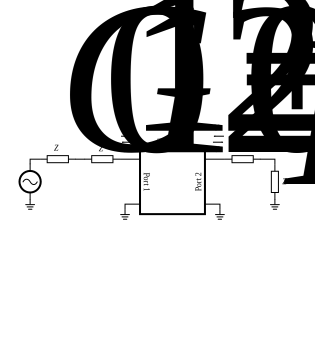
\includegraphics{img/analysis/s_parameter_twoport}
    \caption{S-parameters of a two-port system.}
    \label{fig:twoport}
\end{figure}

The reflection coefficient, $\Gamma$, can more generally be described as an \emph{S-parameter}. The S-parameters describe the ratio between the reflected and incident wave at a given port in a system. Consider a two-port as shown in Figure~\ref{fig:twoport}. Its four S-parameters are defined as follows:
\begin{align*}
    &S_{11} = \frac{V_1^-}{V_1^+} \Bigg|_{V_2^+=0} = \Gamma_1
    &&S_{12} = \frac{V_1^-}{V_2^+} \Bigg|_{V_1^+=0} \\
    &S_{21} = \frac{V_2^-}{V_1^+} \Bigg|_{V_2^+=0}
    &&S_{22} = \frac{V_2^-}{V_2^+} \Bigg|_{V_1^+=0} = \Gamma_2
\end{align*}
It is seen that $S_{11}$ and $S_{22}$ indicate the reflection due to the incident wave on the same port, when no contribution is made from the opposite port, i.e., these are the reflection coefficients of port 1 and 2, respectively. The parameter $S_{21}$ indicates how much of the incident wave on port 1 is coming out of port 2 when no wave is incident on port 2, i.e., this indicates the \emph{transmission coefficient} from port 1 to port 2. Likewise, $S_{12}$ is the transmission coefficient from port 2 to port 1.

The S parameters are easily measured using a Vector Network Analyzer (VNA). The advantage of measuring S-parameters over, e.g., Y-parameters is that all ports are matched during the measurement instead of some being shorted, making odd behavior (like oscillations) less likely \cite{Bowick2007}.

% Smith chart visualization
\begin{figure}[htbp]
    \centering
    \begin{tikzpicture}
        \begin{smithchart}
            \addplot coordinates {(3,0)};
            \path[draw=red] (0pt,0pt) circle (14.4mm);
        \end{smithchart}
    \end{tikzpicture}
    \caption{Smithchart. \fixme{SWR line not accurate\ldots}}
    \label{fig:smithchart}
\end{figure}
An important tool when doing matching, and designing antennas, to a certain $Z_0$ is the smith chart. The smith chart is used for plotting complex, normalized impedances and makes it easy to visually analyze the performance of a matched circuit. A smith chart is shown in Figure~\ref{fig:smithchart}.

The smith chart maps the entire right complex half-plane into a circle, having $0+j0$ all the way to the left and $\infty+j0$ all the way to the right. The y-axis (crossing $x=0$) makes up the circumference of the circle. An impedance is plotted by first finding the resistive (real) part of the impedance on the horizontal line and then following the circular grid-lines up or down for positive or negative reactances, respectively. 

The smith chart shown in Figure~\ref{fig:smithchart} is a normalized smith chart. When matching to $Z_0$, any impedance, $Z$, plotted in the smith chart, must be normalized by $Z_0$:
\begin{equation}
    Z_n = \frac{Z}{Z_0}
\end{equation}
This means that $Z_0$ will always appear at $1+j0$ -- in the center -- of the smith chart, and the goal of the matching is to get the impedance of the antenna (or other circuitry) as close to the center as possible for the desired frequency range.

The impedance bandwidth of an antenna is often given as the bandwidth for which the reflection coefficient, $\Gamma$, is below 0.5 (or \SI{-6}{dB}). It may therefore be advantageous to plot this requirement. In the smith chart, this is plotted as a circle around the center and any point within the circle, is within the bandwidth of the circuit. The \SI{-6}{dB} circle is also shown in Figure~\ref{fig:smithchart}.

% Matching circuitry, L-network, smith chart ``ups and downs'', analytical formulas.

% Tuners: Series capacitor, shunt capacitor, variable inductor?

% Insertion loss, S21 for networks, equivalent series resistance, component Q.

\section{LTE}
In this part an overview of the allocated LTE frequency bands will be provided together with a general description of the lte spectrum.
Furthermore in addition to the allocated LTE bands a more detailed description on the bands covered in this project will be provided.

LTE (Long Term Evolution) is an evolution of the UMTS (Universal Mobile Telecommunications System), HSPA (High Speed Packet Access) and HSPA+ (Evolved High Speed Packet Access) 3G communication standards. HSPA and HSPA+ are upgrades to UMTS for the primary goal to provide higher data rates. The LTE is advertised as a 4G network first commercial services was introduced in 2009 
 
\subsection{LTE Frequency Band Allocation}
\begin{table}[]
\centering
\caption{LTE frequency band allocation \cite{radio2015electronics}}
\label{table:ltefreqband}
\begin{tabular}{|c|c|c|c|c|c|}
\hline
\begin{tabular}[c]{@{}c@{}}LTE\\ band\\ number\end{tabular} & \begin{tabular}[c]{@{}c@{}}Uplink\\ (MHz)\end{tabular} & \begin{tabular}[c]{@{}c@{}}Downlink\\ (MHz)\end{tabular} & \begin{tabular}[c]{@{}c@{}}Width\\ of\\ band \\ spacing\end{tabular} & \begin{tabular}[c]{@{}c@{}}Duplex\\ spacing\\ (MHz)\end{tabular} & \begin{tabular}[c]{@{}c@{}}Band \\ Gap\\ (MHz)\end{tabular} \\ \hline
1                                                           & 1920 - 1980                                            & 2110 - 2170                                              & 60                                                                   & 190                                                              & 130                                                         \\ \hline
2                                                           & 1850 - 1910                                            & 1930 - 1990                                              & 60                                                                   & 80                                                               & 20                                                          \\ \hline
3                                                           & 1710 - 1785                                            & 1805,-1880                                               & 75                                                                   & 95                                                               & 20                                                          \\ \hline
4                                                           & 1710 - 1755                                            & 2110 - 2155                                              & 45                                                                   & 400                                                              & 355                                                         \\ \hline
5                                                           & 824 - 849                                              & 869 - 894                                                & 25                                                                   & 45                                                               & 20                                                          \\ \hline
6                                                           & 830 - 840                                              & 875 - 885                                                & 10                                                                   & 35                                                               & 25                                                          \\ \hline
7                                                           & 2500 - 2570                                            & 2620 - 2690                                              & 70                                                                   & 120                                                              & 50                                                          \\ \hline
8                                                           & 880 - 915                                              & 925 - 960                                                & 35                                                                   & 45                                                               & 10                                                          \\ \hline
9                                                           & 1749.9 - 1784.9                                        & 1844.9 - 1879.9                                          & 35                                                                   & 95                                                               & 60                                                          \\ \hline
10                                                          & 1710 - 1770                                            & 2110 - 2170                                              & 60                                                                   & 400                                                              & 340                                                         \\ \hline
11                                                          & 1427.9 - 1452.9                                        & 1475.9 - 1500.9                                          & 20                                                                   & 48                                                               & 28                                                          \\ \hline
12                                                          & 698 - 716                                              & 728 - 746                                                & 18                                                                   & 30                                                               & 12                                                          \\ \hline
13                                                          & 777 - 787                                              & 746 - 756                                                & 10                                                                   & -31                                                              & 41                                                          \\ \hline
14                                                          & 788 - 798                                              & 758 - 768                                                & 10                                                                   & -30                                                              & 40                                                          \\ \hline
15                                                          & 1900 - 1920                                            & 2600 - 2620                                              & 20                                                                   & 700                                                              & 680                                                         \\ \hline
16                                                          & 2010 - 2025                                            & 2585 - 2600                                              & 15                                                                   & 575                                                              & 560                                                         \\ \hline
17                                                          & 704 - 716                                              & 734 - 746                                                & 12                                                                   & 30                                                               & 18                                                          \\ \hline
18                                                          & 815 - 830                                              & 860 - 875                                                & 15                                                                   & 45                                                               & 30                                                          \\ \hline
19                                                          & 830 - 845                                              & 875 - 890                                                & 15                                                                   & 45                                                               & 30                                                          \\ \hline
20                                                          & 832 - 862                                              & 791 - 821                                                & 30                                                                   & -41                                                              & 71                                                          \\ \hline
21                                                          & 1447.9 - 1462.9                                        & 1495.5 - 1510.9                                          & 15                                                                   & 48                                                               & 33                                                          \\ \hline
22                                                          & 3410 - 3500                                            & 3510 - 3600                                              & 90                                                                   & 100                                                              & 10                                                          \\ \hline
23                                                          & 2000 - 2020                                            & 2180 - 2200                                              & 20                                                                   & 180                                                              & 160                                                         \\ \hline
24                                                          & 1625.5 - 1660.5                                        & 1525 - 1559                                              & 34                                                                   & -101.5                                                           & 135.5                                                       \\ \hline
25                                                          & 1850 - 1915                                            & 1930 - 1995                                              & 65                                                                   & 80                                                               & 15                                                          \\ \hline
26                                                          & 814 - 849                                              & 859 - 894                                                & 30/40                                                                &                                                                  & 10                                                          \\ \hline
27                                                          & 807 - 824                                              & 852 - 869                                                & 17                                                                   & 45                                                               & 28                                                          \\ \hline
28                                                          & 703 - 748                                              & 758 - 803                                                & 45                                                                   & 55                                                               & 10                                                          \\ \hline
29                                                          & n/a                                                    & 717 - 728                                                & 11                                                                   &                                                                  &                                                             \\ \hline
30                                                          & 2305 - 2315                                            & 2350 - 2360                                              & 10                                                                   & 45                                                               & 35                                                          \\ \hline
31                                                          & 452.5 - 457.5                                          & 462.5 - 467.5                                            & 5                                                                    & 10                                                               & 5                                                           \\ \hline
\end{tabular}
\end{table}

From the table it is seen that the allocated LTE bands reaches from \SIrange{452.5}{3600}{MHz}, although the whole spectrum is not covered by the lte, as other communication systems as GSM (2G) and UMTS (3G) etc. also uses band in this frequency range.  

FDD, TDD -- 

broadcast television spectrum around \SI{600}{MHz} has been freed
\cite{Samantha2015tunableAntennas}

 -- Europe band 20, 3, 7 


\subsection{Covered Bands}
In this project the frequencies of interest are \SIrange{700}{960}{MHz}, \SIrange{1710}{2170}{MHz}, \SIrange{2300}{2400}{MHz} and \SIrange{2550}{2650}{MHz}, also as specified in the requirement specification.


\section{User Effects}
\label{se:user_effects}
In this section the user impact on mobile antenna performance will be described, including both effects of the head, hand and the body in general.


Antenna parameters such as efficiency, radiation pattern, impedance etc. will be effected by the user, as the body of the user will look like a lossy and large dielectric body from the antennas point of view. 
The internal antennas that are implemented in every phone today, have a similar performance compared to external stubby antennas, which were used in a numerous of older designs. However this is only if the antennas are measured and compared in free space or next to a phantom head. In practical use a mobile phone with an internal antenna design, will be much more vulnerable to head and hand impacts from the user. The negative performance impact will be there, but will differ from user to user, as things like head and hand size, characteristics, hold position, left or right hand etc. varies from different users. This is of course a drawback in switching from external to internal antennas, but the development also comes with a lot of advantages. The internal antenna provides robust design and normally has higher performance in mechanical tests, such as drop tests, wearing tests etc. as the antenna is placed inside the phone, thus making physical interaction impossible. 
To counteract and minimize the user effect problem to the internal antennas, some basic design guidelines can be followed.

\subsection{Design Guidelines}
An antenna that is placed in the top of the phone, will be more effected by the user in talk mode, as the antenna will be closer to the head. To avoide this a ground plane can be placed between the user and the head in order to create more isolation. However placing the antenna on top of the ground plane decreases the bandwidth significantly, which leads to a, increase in the antenna size to keep the required bandwidth. This is not a reliable solution in mobile phones, as the size requirement of the antennas are very strict as a result of recent phone designs, with bigger screens and smaller cases. A way to solve this problem is to place the antenna in the bottom of the antenna, thus lowering the user effect and makes is possible to place the antenna without the ground plane as isolation. This solution provides a certain ground clearence, which makes it possible to decrease the volume and thickness of the antenna, thus saving place in the mobile phone. 
This design was proven to work by Motorola with there Motorola Razor V3 phone, which was the first phone to use the bottom placed antenna. There were some skeptics to this design, as the bottom of the phone would be placed in the middle of the hand in talk mode. However Motorola proved that theory wrong and therefore many phone manufactors are using there own bottom placed antennas. This solution of course only applies in talk mode, as the head effect is close to zero, when the phone is used in data mode. In data mode the phone is usually held either in horizontal mode with one hand or in vertical mode with two hands. In horizontal mode, given the size of today's smartphones, the hand will be placed around the middle of the phone (depending on the individual user), thus clearing the top and bottom. This indicates that it does not matter whether the antenna is placed in the top or bottom of the phone. In the case of horizontal mode with two hands, the hands covers both the top and the bottom of the phone, 
so in this case it still makes no difference if the antenna is placed in the bottom or in the top of the phone. 


In talk or data (horizontal or vertical) mode, there will still be some negative user effect on the performance. As long as the head or hand is within the near field of the phone, the impact of the user will be significant and needs some attention. Besides following the simple design guidelines, antenna tuning can be used to optimize the performance, when the antennas center frequency is detuned, as a result of the user impact.

\subsection{Recent Measurements}
A recent studie has been carried out in 2014 on user effects of MIMO LTE performance, which is also the antenna design goal of this project. The study is based on time-domain simulations of the user effects of head and hand phantoms in a free space scenario. The phantom hand used is modified, such that the finger can move across the phones backplane, to give more realistic results. The simulations is done in CST (Computer Simulation Technology) using the time-domain solver using FEM (Finite Element Method). Furthermore the antenna is placed in different positions, to evaluate on the user effect for different antenna positions. The different positions and the results of the simulation study, can be seen in Table \ref{tab:usereff_s11} and Table \ref{tab:usereff_radeff}. In Table \ref{tab:usereff_s11} the S-Parameter $S_{11}$ and $S_{22}$ are the reflection coefficient for the antenna at port 1 and 2 respectively and the $S_{21}$ results indicated the correlation between the two antennas. From the results it is clearly seen that the antennas is significally de-tuned in the presens of a user. In the worst case, the reflection coefficient drops from \SI{-8.2}{dB} to \SI{-0.6}{dB}, which is the case for the side mounted antenna. The bottom mounted antenna is the best case, where the reflection coefficient only drops approx. \SI{-2.5}{dB}, which is still a noticable drop. The correlation between the antennas

Finger position !    

\begin{table}[]
  \centering
  \begin{tabular}{|c|c|c|c|c|c|c|}
    \hline
    & \multicolumn{3}{c|}{\textbf{Antennas: Top/Side}} & \multicolumn{3}{c|}{\textbf{Antennas: Bottom/Side}} \\ \hline
                & $S_{11}$        & $S_{22}$        & $S_{21}$       & $S_{11}$         & $S_{22}$         & $S_{21}$             \\ \hline
    \textbf{FS} & -7.9           & -8.2           & -8.4           & -7.9            & -8.2            & -8.4            \\ \hline
    \textbf{P1} & -2.4           & -1.2           & -22.7          & -5.5            & -1.1            & -21.0           \\ \hline
    \textbf{P2} & -4.8           & -1.2           & -22.5          & -5.5            & -0.6            & -22.9           \\ \hline
    \textbf{P3} & -2.0           & -1.2           & -22.8          & -5.1            & -1.8            & -19.7           \\ \hline
    \textbf{P4} & -4.8           & -1.2           & -22.2          & -5.2            & -1.9            & -19.2           \\ \hline
    \textbf{P5} & -1.5           & -1.1           & -22.6          & -4.8            & -2.6            & -19.4           \\ \hline
    \textbf{P6} & -4.3           & -1.1           & -22.5          & -5.0            & -2.0            & -18.5           \\ \hline
  \end{tabular}
  \caption{S-parameter of the two MIMO antennas in free space compared to the user effect of the hand in six different finger positions \cite{Samantha2014UserEff}}
  \label{tab:usereff_s11}
\end{table}

\begin{table}[]
\centering
\begin{tabular}{|c|c|c|c|c|c|c|c|c|}
\hline
            & \multicolumn{4}{c|}{\textbf{Antennas: Top/Side}} & \multicolumn{4}{c|}{\textbf{Antennas: Bottom/Side}} \\ \hline
            & R1         & R2        & T1         & T2         & R1         & R2          & T1         & T2          \\ \hline
\textbf{FS} & -0.2       & -1.1      & -1,0       & -1,9       & -0.2       & -1.1        & -1.0       & -1.9        \\ \hline
\textbf{P1} & -13.4      & -9.2      & -15.8      & -14.8      & -8.9       & -10.9       & -9.6       & -17.0       \\ \hline
\textbf{P2} & -14.1      & -8.6      & -14.7      & -14.6      & -8.6       & -9.7        & -9.0       & -18.5       \\ \hline
\textbf{P3} & -13.3      & -9.3      & -16.2      & -14.9      & -8.7       & -14.4       & -9.7       & -18.5       \\ \hline
\textbf{P4} & -14.3      & -8.9      & -14.9      & -14.9      & -8.6       & -14.4       & -9.6       & -18.2       \\ \hline
\textbf{P5} & -14.0      & -9.6      & -17.6      & -15.5      & -8.9       & -15.2       & -9.9       & -18.8       \\ \hline
\textbf{P6} & -14.0      & -8.8      & -14.6      & -15.0      & -8.7       & -15.4       & -9.7       & -18.1       \\ \hline
\end{tabular}
\caption{Radiation and total efficiency of the two MIMO antennas in free space compared the user effect of the hand in six different finger positions \cite{Samantha2014UserEff}}
\label{tab:usereff_radeff}
\end{table}


User effects of MIMO LTE performance 2014 measurements. \cite{Samantha2014UserEff}
\section{Finite Difference Time Domain}
\label{sec:fdtd}
This section will describe the finite difference time domain method. This is a method for solving Maxwell equations in time domain. A brief introduction to Marxwell's Equations is given, in order to understand the methodology of FDTD. Then the teqniques and ideas behind FDTD are presenten and used on the 1D scalar wave-equation. Then an introduction to the Yee Algorithm, Yee cell and Yee notation is presenten and applied on the 3D Maxwell curl equation. Lastly the key parameters of FDTD are discussed and related to CST Microwavestudio.

\subsection{Introduction to Maxwell's Equations}
Maxwell's equations are a set of equations that describe how electric and magnetic fields propagate. The set of equations consists of Gauss' law, Gauss' Magnetism law, Faraday's law and finally Ampere's law. 

\subsubsection{Gauss' Law}
Gauss' law describes how the electric field behaves around electric charges. Below is Gauss' Law written in point differential-form, the equation states that the divergence of the electric flux density $\bold{D}$ is equal to the volume electric charge density $\rho_V$ \cite{taflove2000computional}. This is that the field around a point $\bold{D}$ is equal to electric charge density $\rho_V$. From this it is found that if there exists an electric charge, the divergence of $\bold{D}$ is nonzero, and only zero when there is no charge present. 

\begin{align}
\nabla \cdot \bold{D} &= \rho_V
\end{align}

\subsubsection{Gauss' Magnetism Law}
Gauss' magnetism law, is much like the previous formula, but for magnetic fields. Basically Gauss' law for magnetism states that a magnetic charge does not exist. This is given in the Equation below \cite{taflove2000computional}. 
\begin{align}
\nabla \cdot \bold{B} &=0
\end{align}
From this it is clear, that there are no magnetic monopoles, the divergence of $\bold{B}$ or $\bold{H}$ fields is always zero and that magnetic fields always flows in closed loops. 

\subsubsection{Faraday's Law}
Faraday's law states that the curl of the $\bold{E}$, is equal to the rate of change of a magnetic field. This is very important in the way that electric ways propagate. This is given in the Equation below \cite{taflove2000computional}. 
\begin{align}
\nabla \times \bold{E} &= - \frac{\partial \bold{B}}{\partial t}
\end{align}

From this equation, it can be seen that a time changing magnetic field gives rise to an E-field circulating around it. Likewise, a circulating E-field causes a time changing magnetic field.   

\subsubsection{Ampere's Law}
Ampere's law, is much like Faraday's law, but for curling magnetic fields. In simple words the Equation below stats that the curl of a magnetic field $\bold{H}$ is given by the rate of change of a electric field $\bold{D}$ termed displacement current density and the electric current density\cite{taflove2000computional}.

\begin{align}
\nabla \times \bold{H} &= \frac{\partial \bold{D}}{\partial t} + \bold{J} 
\end{align}
This is very much symmetric to Faraday's law, with an additional term. However the outcome is the same. That is that a time changing electric field gives rise to an H-field circulating around it and likewise a circulating H-field causes a time changing electric field. From Faraday and Ampere's law it is seen how waves can actually propagate, since a change in an electric field causes a curling magnetic field and so on.    

\subsubsection{Constitutive relations}
Before doing any mathematical manipulations or calculations, it is necessary to have an idea on how the different terms and variables are connected through physical constants. E.g. how the electric flux density is connected to the electric field, which can lead to simplification of calculations later on.

\paragraph{Electric Flux Density:} The electric flux density $\bold{D}$ is related to the electric field $\bold{E}$ by the permittivity measured in Farads per meter. Permittivity is a fundamental parameter of a given material, which affects the propagation of an electric field. Typically it is denoted by $\epsilon$. The relation is given by\cite{taflove2000computional}: 

\begin{align}
  \bold{D} = \epsilon \bold{E}
\end{align}

\paragraph{Magnetic Flux Density:} The magnetic flux density $\bold{B}$ is related to the magnetic field $\bold{H}$ by the permeability measured in Henries per meter. Permeability is a fundamental parameter of a given material, which affects the propagation of a magnetic field. Typically it is denoted by $\mu$. The relation is given by\cite{taflove2000computional}: 

\begin{align}
  \bold{B} = \mu \bold{H}
\end{align}
\paragraph{Electric Current Density:}  The electric current density $\bold{J}$ is related to the electric field $\bold{E}$ by the conductivity measured in Siemens per meter. Permeability is a fundamental parameter of a given material, which affects the current flow in a conductor. Typically it is denoted by $\sigma$. The relation is given by\cite{taflove2000computional}: 

\begin{align}
  \bold{J} = \sigma \bold{E}
\end{align}

\subsection{The 1D Wave Equation}
The wave equation is one of the most basic partial differential equation, which describes how waves propagate. This section will use the 1-dimension wave to describe the method of FDTD. Furthermore it is assumed that

\begin{itemize}
\item The region is free of charge and current: $\bold{J} = \bold{M} = 0$
\item The medium is linear (field-independent)
\item The medium is isotropic (direction-independent)
\item The medium is non-dispersive (frequency-independent)
\end{itemize}
Given these assumptions, Ampere's and Faraday's law can be rewritten as

\begin{align}
  \frac{\partial \epsilon \bold{E}}{\partial t} = \nabla \times \bold{H} - 0 & \implies \frac{\partial \bold{E}}{\partial t} = \frac{1}{\epsilon} \nabla \times \bold{H} \\
\frac{\partial \mu \bold{H}}{\partial t} =  - \nabla \times \bold{E} - 0 & \implies \frac{\partial \bold{H}}{\partial t} = - \frac{1}{\mu} \nabla \times \bold{E}
\end{align}
Expanding E- and H-field into the Cartesian components 

\begin{align}
  \frac{\partial E_x}{\partial t} = \frac{1}{\epsilon} \big(\frac{\partial H_z}{\partial y} - \frac{\partial H_y}{\partial t} \big) \qquad  
  \frac{\partial H_x}{\partial t} = \frac{1}{\mu} \big(\frac{\partial E_z}{\partial y} - \frac{\partial E_y}{\partial t} \big)\\
  \frac{\partial E_y}{\partial t} = \frac{1}{\epsilon} \big(\frac{\partial H_x}{\partial y} - \frac{\partial H_z}{\partial t} \big) \qquad 
  \frac{\partial H_y}{\partial t} = \frac{1}{\mu} \big(\frac{\partial E_x}{\partial y} - \frac{\partial E_z}{\partial t} \big) \\
  \frac{\partial E_z}{\partial t} = \frac{1}{\epsilon} \big(\frac{\partial H_y}{\partial y} - \frac{\partial H_x}{\partial t} \big) \qquad 
  \frac{\partial H_z}{\partial t} = \frac{1}{\mu} \big(\frac{\partial E_y}{\partial y} - \frac{\partial E_x}{\partial t} \big)
\end{align}
which for the 1D case $\frac{\partial}{\partial z} = \frac{\partial}{\partial y} = 0$ simplifies to 

\begin{align}
  \frac{\partial E_x}{\partial t} &= 0 \\
  \frac{\partial E_y}{\partial t} &= - \frac{1}{\epsilon} \frac{\partial H_z}{\partial x}\\
  \frac{\partial E_z}{\partial t} &= \frac{1}{\epsilon} \frac{\partial H_y}{\partial x}
\end{align}
The same steps can be used to get an expression for the H-field. For each direction we can combine the E and H expressions to get the 1D scalar wave equation, e.g. the z-direction\cite{taflove2000computional}: 

\begin{align}
  \frac{\partial^2 E_z}{\partial t^2} = c^2 \frac{\partial^2 E_z}{\partial x^2}
\end{align}
Where $c$ is the speed of light. This equation tells us that an electric field moving in the z-direction, will propagate along the x-axis in time, with a speed of $c$. Going back to the general wave-equation\cite{taflove2000computional}

\begin{align}
  \frac{\partial^2 u}{\partial t^2} = c^2 \frac{\partial^2 u}{\partial x^2}
\end{align}
Since the wave-equation is a second order partial differential equation, it is known to have two linearly independent solutions\cite{taflove2000computional}: 

\begin{align}
  u(x,t) = F(x+ct) + G(x-ct)
\end{align}
Both $F$ and $G$ are known as propagating-wave solutions, where an argument of the form $x+ct$ is a wave moving towards decreasing $x$ and an argument of the form $x-ct$ is a wave moving towards increasing $x$\cite{taflove2000computional}. In order to compute this numerically finite differences are used. Thus the following needs to be approximated using finite-differences 

\begin{align}
  \frac{\partial^2 u(x,t)}{\partial t^2},\frac{\partial^2 u(x,t)}{\partial x^2}
\end{align}

Taylor series expansion is used to approximate the expression at a point $x_i$ using finite differences: $u(x_i) = u(x_i+\Delta x) + u(x_i - \Delta x)$ which then is used to solve the wave-equation by substituting the two central differences into the 1D wave equation. This gives the solution for the latest time step as\cite{taflove2000computional}

\begin{align*}
  u_i^{n+1} =& \left( \frac{c\Delta t}{\Delta x} \right) \left[ u_{i+1}^n - 2u_i^n + u_{i-1}^n \right] + 2u_i^n -u_i^{n-1} \\
             &+ O[(\Delta t)^2] + O[(\Delta x)^2]
\end{align*}

\subsection{Dispersion}
When ever discrete numerical methods are used dispersion must be taken into account. Dispersion in this case can be seen as a variation in wavelength. For the wave equation this depends on the chosen time and space steps\cite{taflove2000computional}. 

\begin{itemize}
\item \textbf{Magic time-step:} $c\Delta t = \Delta x$. No dispersion.
\item \textbf{Very fine mesh:} $\Delta t \rightarrow 0$, $\Delta x \rightarrow 0$. No dispersion.
\item \textbf{Difference 1:} $c\Delta t < \Delta x$. Wavelength smaller in sampled space than in reality.
\item \textbf{Difference 2:} $c\Delta t > \Delta x$. Unstable as $\omega$ is complex. Exponential growth.
\end{itemize}

Generally the magic time-step is only an exact solution in 1D, but it exists for all dimensions but only for one incident angle\cite{taflove2000computional}. It is also seen that finer mesh cells reduces the error term.  

\subsection{The Yee Algorithm}
The Yee algorithm is a set of finite difference equations for Maxwell's curl equation system derived by Kane Yee. This algorithm solves both E- and H-fields in space and time using coupled curl equations instead of solving for one field at a time using the wave equation. Some of the key features of the Yee Algorithm is\cite{taflove2000computional}

\begin{itemize}
\item Both E- and H-field boundaries can be used
\item Solving both E- and H-fields is more robust 
\item Electric and magnetic material properties can be modeled easily
\item Unique field features, e.g. singularities. 
\end{itemize}
The Yee algorithm centers the E- and H-fields in 3D, such that every E-field is surrounded by four curling H-fields and every H-field is surrounded by four curling E-fields. This is illustrated on Figure~\ref{fig:fdtd-grid}, each cell referred to as the Yee-cell, a single Yee cell is shown in Figure~\ref{fig:yee-cell}. The arrangement of the electric and magnetic fields implicitly enforce Gauss' Law and Gauss' Magnetic Law, which makes the Yee mesh divergence free with respect to the E- and H-fields\cite{taflove2000computional}.  

\begin{figure}
    \centering
    \begin{subfigure}[b]{0.49\textwidth}
      \centering
        \includegraphics[scale=0.3]{img/analysis/fdtd_mesh}
        \caption{A Yee FDTD grid}
        \label{fig:fdtd-grid}
    \end{subfigure}
    ~
    \begin{subfigure}[b]{0.49\textwidth}
      \centering
        \includegraphics[scale=0.7]{img/analysis/yee_3d}
        \caption{A single Yee cell}
        \label{fig:yee-cell}
    \end{subfigure}
    \caption{Spatial interpetation of the Yee Algorithm}
    \label{fig:space-yee-algorithm}
\end{figure}

The centering of the E- and H-fields in time, is often termed the leapfrog method. This time stepping is fully explicit, and thus avoiding problems with simultaneous equations and matrix inversion. This leapfrog method is shown on Figure~\ref{fig:leap_frog} 

\begin{figure}[htbp]
    \centering
    \includegraphics[scale=0.7]{img/analysis/leap_frog}
    \caption{Leap-frog method illustrated on the time line}
    \label{fig:leap_frog}
\end{figure}

To keep an overview Yee, created the following notation which is useful when considering 3D FDTD equations

\begin{align}
  u_X (i \Delta x , j \Delta y, k \Delta z, n \Delta t) = u^n_{X_{i,j,k}}
\end{align}

%http://www.ualr.edu/wirelesslab/fdtd/fdtd3.pdf
\subsubsection{Finite Difference of Maxwell's Equations in 3D}
For completeness the previous ideas and notation can now be used to derive a numerical approximation of Maxwell's Curl Equations in 3D. The derivations will not be shown here, and only the solution for a single Cartesian component will be given here, due to its complexity. As an example the approximation for $E_x$ is shown below\cite{taflove2000computional}: 

\begin{align}
  &E_x |^{n+1/2}_{i,j+1/2,k+1/2} = \big( \frac{1-\frac{\sigma_{i,j+1/2,k+1/2} \Delta t}{2\epsilon_{i,j+1/2,k+1/2}}}{1+\frac{\sigma_{i,j+1/2,k+1/2} \Delta t}{2\epsilon_{i,j+1/2,k+1/2}}} \big) E_x |^{n-1/2}_{i,j+1/2,k+1/2}  + \\ &\big(  \frac{\frac{\Delta t}{\epsilon_{i,j+1/2,k+1/2}}}{1+\frac{\sigma_{i,j+1/2,k+1/2} \Delta t}{2\epsilon_{i,j+1/2,k+1/2}} }    \big) \big( \frac{H_z |^n_{i,j+1,k+1/2} - H_z |^n_{i,j,k+1/2} }{\Delta y} - \frac{H_y |^n_{i,j+1/2,k+1} - H_y |^n_{i,j+1/2,k} }{\Delta z} -J_{source}|^n_{i,j+1/2,k+1/2}  \big)
\end{align}

As seen the equations quickly become large and hard to handle, however to fully extend this to 3D this would have to be done for all the the Cartesian coordinates for both E- and H-fields. 

\subsection{Absorbing Boundary Conditions}
Since many geometries of interest are defined in open regions, e.g. antennas, where the spatial domain is unbounded. Since computers have limited storage, it is needed to find a suitable boundary condition on the outer perimeter of the domain $\Omega$ in order to simulate to infinity. Thus it is needed to find a boundary condition that allows outward propagating numerical wave to exit the outer perimeter of $\Omega$, without spurious reflections from the outgoing waves. 

One way of achieving the absorbing boundary condition is by terminating the outer boundary with an absorbing material, which is analogous to the method used in anechoic chambers. For this perfectly matched layer (PML) is used, which is derived by Berenger. This allows plane waves of arbitrary incidence, polarization and frequency to be matched at the boundary. PML usually gives a back-reflection in the order of $\approx 10^{-6}$--$10^{-8}$.\cite{taflove2000computional}

\subsection{FDTD Parameters and Relation to CST}
For all simulations in this report CST microwave studio is being used. The following will try to connect the FDTD theory to the parameters in CST. Even though CST uses Finite Integration Technique (FIT) instead of finite differences. FIT share the structure of FDTD, but using the Maxwell's Equations on integral form. The advantage of FIT is that is uses less memory and it is allows for easier code implementation of some features. Besides this most of the basic parameters are the same. 

\subsubsection{Cell Size and Meshing}
The coice of cell size is very important when doing FDTD simulations. A general rule of thumb is that a cell should be much less than the smallest wavelength, it is often said that 10 cells per wavelength is sufficient, that is the cell size should be $\lambda/10$. In advanced FDTD simulations an adaptive meshing is often used, where even smaller cells are used in dense materials with high field locations, and then large cells outside these areas. When doing this it is also very important not to change the cell size too much compared to the neighbor cells. It is also important
that the cell size are small enough to approximate the geometry which is to be modeled accurately. Geometries such as circles are being approximated with rectangular cells, this causes a ``staircase effect'' on the object, and the representation can be inaccurate if the cell sizes used are too large. 

Another rule of thumb, which can help assessing the right cell size is that the smallest mechanical item of the structure is to be approximated by at least two cells. The rule of thumb says that\cite{kunz1993fdtd}:
\begin{align}
    \Delta = \frac{d_{\text{min}}}{N_d} 
\end{align}
where 
\begin{where}
\item[$\Delta$] Is the length/width/height of the cell.
\item[$d_{\text{min}}$] Smallest physical dimension.
\item[$N_d$] Oversampling factor -- should be $\geq 1$.
\end{where}


\subsubsection{Time Step Size}
The time step size is another parameter that has to be chosen with care, when doing FDTD simulations. The time step should be small enough, such that at any point a wave should not pass through more than one cell.  Calculating the time step is dependent on the cell size and dimensions and the propagation speed.  The time step for the 3D rectangular grid can be calculated as:
\begin{align}
   \Delta t &= \frac{1}{c \sqrt{\frac{1}{(\Delta x)^2}+\frac{1}{(\Delta y)^2}+\frac{1}{(\Delta z)^2}}} \\
            &= \frac{1}{c \sqrt{\frac{3}{\Delta^2}}} \\
            &= \frac{\Delta}{c \sqrt{3}} \label{eq:deltat}           
\end{align}
where:
\begin{where}
\item [$c$] Speed of light.
\item [$\Delta = \Delta x = \Delta y = \Delta z$] Size of the cell side for rectangular cell.
\end{where}
The step size should also be reduced for the materials with conductivity higher then zero. If the time step is chosen to be larger than given in Equation~\ref{eq:deltat} instabilities can occur \cite{kunz1993fdtd}.   

\subsubsection{Accuracy and time limit}
These terms are taking from CST microwave studio, and are figures that limit the simulation either when a certain accuracy criteria has been met or when it has been simulation for a certain amount of time. In practice it is not wanted that a simulation is to be stopped due to a given time limit, therefor this limit is often set to a very large number. In CST accuracy is a figure that describes how much energy is left in the system. The accuracy setting stops the simulation when a certain energy level within the structure has decreased to a chosen level. 

\section{Problem Statement}
\label{sec:problem_statement}
The problem statement, which will be investigated in this report, is formulated as the following:
\begin{quote}
    \itshape
    How can a pair of MIMO antennas for LTE handsets be designed so that all bands from \SI{700}{MHz} to \SI{960}{MHz} and from \SI{1710}{MHz} to \SI{2650}{MHz} are covered with a total efficiency above \SI{50}{\%} using a tunable MEMS capacitor, and how does a small ground clearance -- the distance between the antenna element and the ground plane -- affect the performance?
\end{quote}
The further specifications for the design will be described next in the requirement specification.


% Requirements
\chapter{Requirements Specification}
\label{cha:reqspec}

\section{Functional Requirements}
\noindent
\begin{tabularx}{\linewidth}{|l|X|}
    \hline
    ID & Requirement \\
    \hline
    \freq{dualband} & The antenna system must consist of two single-feed dual-band antennas covering the bands described in Requirement~\sreqref{fbands}. \\
    \freq{updownlink} & Each antenna must cover both uplink and downlink at the same time for each required LTE band.\\
    \freq{usereffect} & Must be able to re-tune any detuning due to user effects. \\
    \freq{matching} & Must have a simple matching network, containing a variable capacitor for tuning inside the specified bands.\\
    \freq{wispry} & Must use a wiSpry WS1040 MEMS variable capacitor chip in the matching network.\\
    \hline
\end{tabularx}

\section{Specific Requirements}
\noindent 
\begin{tabularx}{\linewidth}{|l|l|X|}
    \hline
    ID & Specification & Requirement \\
    \hline
    \sreq{fbands} & Frequency bands\slash tunable range & \num{700}--\SI{960}{MHz}, \num{1710}--\SI{2170}{MHz}, \num{2300}--\SI{2400}{MHz}, \num{2550}--\SI{2650}{MHz} \\
    \sreq{bandwidthlow} & Minimum tunable bandwidth (\num{700}--\SI{960}{MHz}) & \SI{80}{MHz} (band 8) \\
    \sreq{bandwidthhigh} & Minimum tunable bandwidth (\num{1710}--\SI{2650}{MHz}) & \SI{720}{MHz} (band 15) \\
    \sreq{physdim} & Physical dimensions & External: $70\times140\times7$\,\si{mm\cubed}, PCB: $55\times120\times1.6$\,\si{mm\cubed} (FR-4)\\
    \sreq{copper} & Ground plane copper thickness & \SI{0.035}{mm} \\
    \sreq{retloss} & In-band return loss (impedance bandwidth) & $\text{RL} > \SI{6}{dB}$\\
    \sreq{correlation} & In-band correlation between antenna elements (correlation bandwidth) & $\rho_e < 0.5$\\
    \sreq{efficiency} & In-band total efficiency in free-space (efficiency bandwidth)  & $>\SI{50}{\%}$ \\
    \sreq{sar} & Maximum SAR & \SI{2}{W\per kg} averaged over \SI{10}{g} of tissue\\
    \sreq{tunable} & Tunable capacitor range (WS1040)& \SI{0.3}{pF} to \SI{2.9}{pF} in steps of \SI{0.2}{pF} (\SI{0.1}{pF} minimum)  \\
    \sreq{ltepower} & Reference power level  & \SI{23}{dBm} (\SI{0.2}{W})\\
    \hline
\end{tabularx}



% Testspecification
\chapter{Testspecification}
\subsubsection{Test of Requirement~\sreqref{fbands}---Frequency Bands/Tunable Range}
The frequency spectrum and the tunable range is tested by measuring the S11 and S22 parameters, using a VNA, for the top and side antenna respectively. The tunable range is done accordingly to requirement \sreqref{tunable} using a variable capacitor in the range \SI{0.3}{pF} to \SI{2.9}{pF} in steps of \SI{0.2}{pF} (\SI{0.1}{pF} minimum). 
\subsubsection{Test of Requirement~\sreqref{bandwidthlow}---Minimum Tunable Bandwidth in the Low Band}
The minimum required bandwidth in the low band  is measured as requirement~\sreqref{fbands}. The minimum required bandwidth is measured from the highest achievable bandwidth when sweeping each capacitor accordingly to requirement \sreqref{tunable}.

\subsubsection{Test of Requirement~\sreqref{bandwidthhigh}---Minimum Tunable Bandwidth in the High Band}
The minimum required bandwidth in the high band is measured as requirement~\sreqref{fbands}. The minimum required bandwidth is measured from the highest achievable bandwidth when sweeping each capacitor accordingly to requirement \sreqref{tunable}.

\subsubsection{Test of Requirement~\sreqref{bandwidthhigh}---Physical Dimensions}
The physical dimensions of the PCB, antenna and the external limitations are measured by a measuring tape. 

\subsubsection{Test of Requirement~\sreqref{copper}---Copper Thickness} This requirement is not tested, as the chosen PCB has a copper thickness of \SI{0.035}{mm}.

\subsubsection{Test of Requirement~\sreqref{correlation}---Correlation Between Antenna Elements}


\subsubsection{Test of Requirement~\sreqref{efficiency}---Total Efficiency in Free-Space}

\subsubsection{Test of Requirement~\sreqref{sar}---Maximum SAR}


\subsubsection{Test of Requirement~\sreqref{tunable}---Physical Dimensions} This requirement is not tested, as the variable capacitor chip is chosen as a wiSpry WS1040 MEMS chip accordingly to requirement~\freqref{wispry}. 

\cite{cita2015}

% Technical solution
\chapter{Post Processing}
\label{cha:postproc}

In this chapter, the libraries for post processing data from CST and Satimo will be described. The libraries are written in Python. By the end of the chapter, usage examples will be given.

\section{Data Format}
The trx files, from Satimo Passive Measurement, contain data formatted in four columns:
\begin{enumerate}
    \item Horizontal polarization, real part.
    \item Horizontal polarization, imaginary part.
    \item Vertical polarization, real part.
    \item Vertical polarization, imaginary part.
\end{enumerate}
Each column contains 
\begin{equation}
    n_r =  n_f \times n_a \times n_e
\end{equation}
where
\begin{where}
\item[$n_r$] Total number of rows per column.
\item[$n_f$] Number of different frequencies in the measurement.
\item[$n_a$] Number of azimuth coordinates (usually 8).
\item[$n_e$] Number of elevation coordinates (usually 15).
\end{where}
The first $n_a \times n_e$ rows are for the first frequency and the next $n_a \times n_e$ rows are for the second frequency. Within this, the first $n_e$ rows are for the first azimuth angle and so on.

To get a better overview, the basic format for the following libraries is a $\theta \times \phi$-matrix like the following:
\begin{equation}
    M = \begin{bmatrix}
        m_{1,1} & m_{1,2} & \dots & m_{1,n} \\
        m_{2,1} & m_{2,2} & \dots & m_{2,n} \\
        \vdots & \vdots & & \vdots \\
        m_{m,1} & m_{m,2} & \dots & m_{m,n}
    \end{bmatrix}
\end{equation}
The data is rearranged to have $\phi$ go from \ang{0} to \ang{360} and $\theta$ from \ang{0} to \ang{180} as shown in Table~\ref{tab:matrixformat}.

\begin{table}[htbp]
    \centering
    \begin{tabular}{|l|c|c|}
        \hline
        Elements & $\theta$ & $\phi$ \\
        \hline
        $m_{1,1}$ & \ang{0} & \ang{0} \\
        $m_{1,n}$ & \ang{0} & $\ang{360}$ \\
        $m_{m,1}$ & \ang{180}$^{\dagger}$ & \ang{0} \\
        \hline
    \end{tabular}
    \caption{Format of $\theta\times\phi$-matrix. $^{\dagger}$For Satimo measurements, this is $180-22.5=\ang{157.5}$ because of the blind spot in the bottom.}
    \label{tab:matrixformat}
\end{table}

\section{Antenna Design 1 -- Monopole}

\begin{figure}[htbp]
    \begin{subfigure}[b]{0.49\linewidth}
        \centering
        \includegraphics{img/tech_sol/monopole/tech_drawing}
        \caption{Technical drawing.}
        \label{fig:ant1technical}
    \end{subfigure}
    \hfill
    \begin{subfigure}[b]{0.49\linewidth}
        \centering
        \includegraphics{img/tech_sol/schematic_tuning_1}\\[1cm]
\footnotesize
        \begin{tabular}{|l|l|l|l|}
            \hline
            & $C_1$ & $L_1$ & $C_2$ \\
            \hline
            Top antenna & \SI{3.02}{pF} & \SI{7.99}{nH} & $[0.3,2.9]\,$pF\\
            Side antenna & \SI{1.81}{pF} & \SI{5.27}{nH} & $[0.3,2.9]\,$pF\\
            \hline
        \end{tabular}
        \caption{Tuning/matching circuit.}
        \label{fig:ant1_tuning}
    \end{subfigure}
    \caption{Technical drawing and tuning circuit for the antenna.  The matching circuit is applied for both the top and the side antenna.}
    \label{fig:ant2techschem}
\end{figure}

%Single antenna description
The antenna design for both antennas is shown in Figure \ref{fig:an1technical}. Both antennas is designed from a basic folded monopole structure with 2 arms one for the low band and one for the high band. The antennas are almost identical with a few changes as a result of the restrictions on the ground clearance.
The antennas are designed to take full advantage of the ground clearance requirements in all directions. This is done in order to obtain the highest possible bandwidth in the low band and high band. 


%MIMO
Going from the top antenna to the side antenna the ground clearance decreases from \SI{10}{mm} to \SI{7}{mm}. To compensate for the decrease in ground clearance the length of both the low band and high band arms are adjusted to meet the bandwidth requirements.

\begin{figure}[htbp]
   \begin{subfigure}[b]{0.32\linewidth}
        \centering
        \includegraphics[width=\linewidth]{img/tech_sol/monopole/sc_800}
        \caption{Surface current for \SI{800}{MHz}}
        \label{fig:ant1_sc800}
    \end{subfigure}
    \hfill
    \begin{subfigure}[b]{0.32\linewidth}
        \centering
        \includegraphics[width=\linewidth]{img/tech_sol/monopole/sc_1800}
        \caption{Surface current for \SI{1800}{MHz}}
        \label{fig:ant1_sc1800}
    \end{subfigure}
    \hfill
    \begin{subfigure}[b]{0.32\linewidth}
        \centering
        \includegraphics[width=\linewidth]{img/tech_sol/monopole/sc_2400}
        \caption{Surface current for \SI{2400}{MHz}}
        \label{fig:ant1_sc2400}
    \end{subfigure}
    \caption{Surface currents at each resonance with $C_2=\SI{0.3}{pF}$.}
    \label{fig:ant1_sc}
\end{figure}

\begin{figure}[htbp]
    \centering
    \includegraphics{img/tech_sol/monopole/ant1_sparam}
    \caption{S-parameters with $C_2=\SI{0.3}{pF}$ for both antennas.}
    \label{fig:ant1surfaces}
\end{figure}

The S11 and S22 sweeps \ref{fig:sparam_mono} shows that both antennas almost covers the desired bandwidth specified in the requirements \ref{cha:reqspec}. However at approx. \SI{2500}{MHz} to \SI{2650}{MHz} both antennas are \SI{-1}{dB} to \SI{-3}{dB} lower than required. The return loss from the side antenna  
\ref{fig:ant1_s22} also shows a lower level that desired, at approx \SI{-5}{dB}. From the requirement specification \ref{cha:reqspec} it is specified that for the low band the minimum channel bandwidth should be \SI{80}{MHz} and for the high band \SI{720}{MHz}. The channel bandwidth for both antennas are shown in Table. \ref{tab:asd}

\subsection{Bandwidth}

    \begin{table}
        \centering
        \begin{tabular}{|l|l|r|r|r|}
            \hline
            Antenna & Band & Start [MHz] & Stop [MHz] & Bandwidth [MHz] \\
            \hline
            Top     & Low  & 680         & 1011       & 331 \\
            Side    & Low  & 818         & 909        & 91 \\
            \hline
            Top     & High & 1590        & 2527       & 937 \\
            Side    & High & 1850        & 2533       & 683 \\
            \hline
        \end{tabular}
        \caption{Maximum bandwidth obtained in the low and high band for the top and the side antenna, respectively.}
        \label{tab:bw_sol2}
    \end{table}

\begin{figure}[htbp]
   \begin{subfigure}[b]{0.49\linewidth}
        \centering
        \includegraphics{img/tech_sol/monopole/s11}
        \caption{S11 plot for the bottom antenna.}
        \label{fig:ant1_s11}
    \end{subfigure}
    \hfill
    \begin{subfigure}[b]{0.49\linewidth}
        \centering
        \includegraphics{img/tech_sol/monopole/s22}
        \caption{S22 plot for the side antenna.}
        \label{fig:ant1_s22}
    \end{subfigure}
~
    \begin{subfigure}[b]{0.49\linewidth}
        \centering
        \includegraphics{img/tech_sol/monopole/s21-s11}
        \caption{$S_{21}$ with $C_2$ = \SI{0.3}{pF} and $C_1$ varying from \SI{0.3}{pF} to \SI{2.9}{pF}.}
        \label{fig:ant1_s11}
    \end{subfigure}
    \hfill
    \begin{subfigure}[b]{0.49\linewidth}
        \centering
        \includegraphics{img/tech_sol/monopole/s21-s22}
        \caption{$S_{21}$ with $C_2$ = \SI{0.3}{pF} and $C_1$ varying from \SI{0.3}{pF} to \SI{2.9}{pF}.}
        \label{fig:ant1_s22}
    \end{subfigure}
    \caption{Parameter sweep for tuning the shunt capacitor of each antenna, $C_1$ and $C_2$ for port 1 and 2, respectively. Port 1 is the top antenna and port 2 is the side antenna.}
    \label{fig:sparam_mono}
\end{figure}



\section{Antenna Design 2 -- Hybrid Triangle Beast}

\begin{figure}[htbp]
    \begin{subfigure}[b]{0.49\linewidth}
        \centering
        \includegraphics{img/tech_sol/trianglefeed/technical}
        \caption{Technical drawing.}
        \label{fig:ant2technical}
    \end{subfigure}
    \hfill
    \begin{subfigure}[b]{0.49\linewidth}
        \centering
        \includegraphics{img/tech_sol/schematic_tuning_1}
        \caption{Tuning/matching circuit.}
        \label{fig:ant2schematic}
    \end{subfigure}
    \caption{Technical drawing and tuning circuit for the antenna.  The antennas are built on FR-4 board using \SI{35}{\micro\meter} copper. There is a matching circuit as shown for each of the two feeds.}
    \label{fig:ant2techschem}
\end{figure}


\section{Antenna Design 3 - Broken Arrow}


\chapter{User Efficiency Simulations}

\begin{figure}[htbp]%{0.49\linewidth}
  \centering
  \includegraphics{img/tech_sol/monopole/sol1_sar}
  \caption{SAR simulation setup}
  \label{fig:ant1_sar}
\end{figure}

\begin{itemize}
\item Meshcells approx $15500000$
\end{itemize}


\section{Antenna Design 1 -- Monopole}



\section{Antenna Design 2 -- Triangle-Feed Antenna}
In this section, the results from Section~\ref{sec:techsol_triang} will be repeated, having the phone in read mode, play mode, and talk mode. Additionally, the maximum SAR value, recorded in the users head, will be simulated. The antenna positions, for each use case, are shown in Figure~\ref{fig:triang_positions}.

\begin{figure}[htbp]
    \centering
    \begin{subfigure}[b]{0.24\linewidth}
        \centering
        \includegraphics[width=\linewidth,height=4cm,keepaspectratio]{img/tech_sol/trianglefeed/read_mode/3d.PNG}
        \caption{Read mode.}
    \end{subfigure}
    \begin{subfigure}[b]{0.24\linewidth}
        \centering
        \includegraphics[width=\linewidth,height=4cm,keepaspectratio]{img/tech_sol/trianglefeed/play_mode/3d.PNG}
        \caption{Play mode.}
    \end{subfigure}
    \begin{subfigure}[b]{0.24\linewidth}
        \centering
        \includegraphics[width=\linewidth,height=4cm,keepaspectratio]{img/tech_sol/trianglefeed/talk_mode/3d.PNG}
        \caption{Talk mode.}
    \end{subfigure}
    \begin{subfigure}[b]{0.24\linewidth}
        \centering
        \includegraphics[width=\linewidth,height=4cm,keepaspectratio]{img/tech_sol/trianglefeed/sar/3d.PNG}
        \caption{SAR.}
    \end{subfigure}
    \caption{Antenna position for each user effect simulation.}
    \label{fig:triang_positions}
\end{figure}

\FloatBarrier
\subsection{Read Mode}
The S-parameters with the tunable capacitors set to their minima are shown in Figure~\ref{fig:triang_sparam_read}. It is seen that that the low band of the side antenna has been tuned down to around the middle of the low band. As it is not possible to tune the resonance further upwards, the bands around \SI{960}{MHz} are not covered at greater than \SI{6}{dB} return loss. The high band is still almost covered at around \SI{5}{dB} return loss. The top antenna, on the other hand, almost covers both the low and the high band simultaneously.

The S-parameters, when sweeping the tunable capacitors, are shown in Figure~\ref{fig:tiang_sparam_sweep_read}. The maximum impedance-bandwidths are summed up in Table~\ref{tab:bw_sol2read}. From this it is again clear that only the top antenna is able to cover the high end of the low band. None of the antennas can cover the high band at \SI{6}{dB} return loss. However, as they can cover the high band at greater than \SI{5}{dB}, this is not considered a problem.

The correlation between the antennas, when sweeping the tunable capacitors, are shown in Figure~\ref{fig:corr_sol2_read}. The correlation is, for frequencies above \SI{750}{MHz}, below 0.5 when sweeping the top antenna. When sweeping the side antenna, the correlation remains below 0.5 for all capacitor settings. The correlation has dropped significantly from the free-space simulation in Figure~\ref{fig:corr_sol2}.

The efficiencies for each antenna, when sweeping the tuning capacitors, are shown in Figure~\ref{fig:eff_sol2read}. It is seen that the efficiency, generally, has decreased from the free space simulation in Chapter~\ref{cha:nousersim}. At  \SI{-3}{dB} efficiency, there is no bandwidth left. At \SI{-6}{dB}, the most of the bands can be covered except at the lower part of the low band for the side antenna where the efficiency decreases to a maximum of \SI{-7}{dB}. The efficiency in the high band is generally higher than in the low band.

\begin{figure}[htbp]
    \centering
    \includegraphics{img/tech_sol/trianglefeed/read_mode/sparams.pdf}
    \caption{Triangular feed antenna in read mode. S-parameters with both tuning capacitors fixed at \SI{0.3}{pF}.}
    \label{fig:triang_sparam_read}
\end{figure}

\begin{table}[htbp]
    \centering
    \begin{tabular}{|l|l|r|r|r|}
        \hline
        Antenna & Band & Start [MHz] & Stop [MHz] & Bandwidth [MHz] \\
        \hline
        Top     & Low  & 570         & 2583       & 2013 \\
        Side    & Low  & 779         & 891        & 112  \\
        \hline
        Top     & High & 570         & 2583       & 2013 \\
        Side    & High & 1506        & 2623       & 1117 \\
        \hline
    \end{tabular}
    \caption{Triangle feed antenna in read mode. Maximum bandwidth obtained in the low and high band for the top and the side antenna, respectively. It is seen that, for the low capacitor settings on the top antenna, both the low and high band are covered at the same time.}
    \label{tab:bw_sol2read}
\end{table}

\begin{figure}[htbp]
   \begin{subfigure}[b]{0.49\linewidth}
        \centering
        \includegraphics{img/tech_sol/trianglefeed/read_mode/Csh1s11.pdf}
        \caption{$S_{11}$, sweeping $C_1$ and fixing $C_2$.}
    \end{subfigure}
    \hfill
    \begin{subfigure}[b]{0.49\linewidth}
        \centering
        \includegraphics{img/tech_sol/trianglefeed/read_mode/Csh2s22.pdf}
        \caption{$S_{22}$, sweeping $C_1$ and fixing $C_2$.}
    \end{subfigure}
    \\
    \begin{subfigure}[b]{0.49\linewidth}
        \centering
        \includegraphics{img/tech_sol/trianglefeed/read_mode/Csh1s21.pdf}
        \caption{$S_{21}$, sweeping $C_1$ and fixing $C_2$.}
    \end{subfigure}
    \hfill
    \begin{subfigure}[b]{0.49\linewidth}
        \centering
        \includegraphics{img/tech_sol/trianglefeed/read_mode/Csh2s21.pdf}
        \caption{$S_{21}$, sweeping $C_2$ and fixing $C_1$.}
    \end{subfigure}
    \caption{Triangle feed antenna in read mode. Parameter sweep for tuning the shunt capacitor of each antenna, $C_1$ and $C_2$ for port 1 and 2, respectively. Port 1 is the top antenna and port 2 is the side antenna.}
    \label{fig:tiang_sparam_sweep_read}
\end{figure}

% Correlation
\begin{figure}[htbp]
    \centering
    \begin{subfigure}{0.49\linewidth}
        \includegraphics{img/tech_sol/trianglefeed/read_mode/correlation_Csh1-sweep}
        \caption{Sweeping $C_1$ and fixing $C_2$.}
    \end{subfigure}
    \hfill
    \begin{subfigure}{0.49\linewidth}
        \includegraphics{img/tech_sol/trianglefeed/read_mode/correlation_Csh2-sweep}
        \caption{Sweeping $C_2$ and fixing $C_1$.}
    \end{subfigure}
    \caption{Triangle feed antenna in read mode. Correlation between antennas then sweeping tuning capacitors. Here, $C_1$ and $C_2$ are the tuning capacitor for the top and side antenna, respectively.}
    \label{fig:corr_sol2_read}
\end{figure}

% Efficiency
\begin{figure}[htbp]
    \centering
    \begin{subfigure}{0.49\linewidth}
        \centering
        \includegraphics{img/tech_sol/trianglefeed/read_mode/efficiency-ac1-Csh1.pdf}
        \caption{Top antenna. Sweeping $C_1$, fixing $C_2$.}
    \end{subfigure}
    \hfill
    \begin{subfigure}{0.49\linewidth}
        \centering
        \includegraphics{img/tech_sol/trianglefeed/read_mode/efficiency-ac2-Csh2.pdf}
        \caption{Side antenna. Sweeping $C_2$, fixing $C_1$.}
    \end{subfigure}
    \caption{Triangle feed antenna in read mode. Efficiency for each antenna when sweeping the tuning capacitors. Here, $C_1$ and $C_2$ are the tuning capacitor for the top and side antenna, respectively.}
    \label{fig:eff_sol2read}
\end{figure}


\FloatBarrier
\subsection{Play Mode}

The S-parameters with the tunable capacitors set to their minima are shown in Figure~\ref{fig:triang_sparam_play}. Here, both the top and side antennas have been tuned down. As for read mode, the side antenna can only cover the lower half of the low band whereas the top antenna can cover cover the lower band at greater than \SI{5}{dB} return loss.

The S-parameters, when sweeping the tunable capacitors, are shown in Figure~\ref{fig:tiang_sparam_sweep_play}. The maximum impedance-bandwidths are summed up in Table~\ref{tab:bw_sol2play}. It is seen, that both antennas almost cover the high band. The tunable bandwidth is still large enough to cover the LTE bands in the low band.

The correlation between the antennas, when sweeping the tunable capacitors, are shown in Figure~\ref{fig:corr_sol2_play}. The correlation is similar to that of the read mode.

The efficiencies for each antenna, when sweeping the tuning capacitors, are shown in Figure~\ref{fig:eff_sol2play}. Compared to the read mode, the high band efficiency of the top antenna has decreased more than the low band efficiency. The side antenna is very similar to the read mode results.

\begin{figure}[htbp]
    \centering
    \includegraphics{img/tech_sol/trianglefeed/play_mode/sparams.pdf}
    \caption{Triangular feed antenna in play mode. S-parameters with both tuning capacitors fixed at \SI{0.3}{pF}.}
    \label{fig:triang_sparam_play}
\end{figure}

\begin{table}[htbp]
    \centering
    \begin{tabular}{|l|l|r|r|r|}
        \hline
        Antenna & Band & Start [MHz] & Stop [MHz] & Bandwidth [MHz] \\
        \hline
        Top     & Low  & 629         & 928        & 299  \\
        Side    & Low  & 780         & 881        & 101  \\
        \hline
        Top     & High & 1379        & 2703       & 1324 \\
        Side    & High & 1388        & 2559       & 1171 \\
        \hline
    \end{tabular}
    \caption{Triangle feed antenna in play mode. Maximum bandwidth obtained in the low and high band for the top and the side antenna, respectively. The bandwidth for the side antennas high band is ignoring the slight rise above \SI{-6}{dB} in the middle of the high band.}
    \label{tab:bw_sol2play}
\end{table}

\begin{figure}[htbp]
   \begin{subfigure}[b]{0.49\linewidth}
        \centering
        \includegraphics{img/tech_sol/trianglefeed/play_mode/Csh1s11.pdf}
        \caption{$S_{11}$, sweeping $C_1$ and fixing $C_2$.}
    \end{subfigure}
    \hfill
    \begin{subfigure}[b]{0.49\linewidth}
        \centering
        \includegraphics{img/tech_sol/trianglefeed/play_mode/Csh2s22.pdf}
        \caption{$S_{22}$, sweeping $C_1$ and fixing $C_2$.}
    \end{subfigure}
    \\
    \begin{subfigure}[b]{0.49\linewidth}
        \centering
        \includegraphics{img/tech_sol/trianglefeed/play_mode/Csh1s21.pdf}
        \caption{$S_{21}$, sweeping $C_1$ and fixing $C_2$.}
    \end{subfigure}
    \hfill
    \begin{subfigure}[b]{0.49\linewidth}
        \centering
        \includegraphics{img/tech_sol/trianglefeed/play_mode/Csh2s21.pdf}
        \caption{$S_{21}$, sweeping $C_2$ and fixing $C_1$.}
    \end{subfigure}
    \caption{Triangle feed antenna in play mode. Parameter sweep for tuning the shunt capacitor of each antenna, $C_1$ and $C_2$ for port 1 and 2, respectively. Port 1 is the top antenna and port 2 is the side antenna.}
    \label{fig:tiang_sparam_sweep_play}
\end{figure}

% Correlation
\begin{figure}[htbp]
    \centering
    \begin{subfigure}{0.49\linewidth}
        \includegraphics{img/tech_sol/trianglefeed/play_mode/correlation_Csh1-sweep}
        \caption{Sweeping $C_1$ and fixing $C_2$.}
    \end{subfigure}
    \hfill
    \begin{subfigure}{0.49\linewidth}
        \includegraphics{img/tech_sol/trianglefeed/play_mode/correlation_Csh2-sweep}
        \caption{Sweeping $C_2$ and fixing $C_1$.}
    \end{subfigure}
    \caption{Triangle feed antenna in play mode. Correlation between antennas then sweeping tuning capacitors. Here, $C_1$ and $C_2$ are the tuning capacitor for the top and side antenna, respectively.}
    \label{fig:corr_sol2_play}
\end{figure}

% Efficiency
\begin{figure}[htbp]
    \centering
    \begin{subfigure}{0.49\linewidth}
        \centering
        \includegraphics{img/tech_sol/trianglefeed/play_mode/efficiency-ac1-Csh1.pdf}
        \caption{Top antenna. Sweeping $C_1$, fixing $C_2$.}
    \end{subfigure}
    \hfill
    \begin{subfigure}{0.49\linewidth}
        \centering
        \includegraphics{img/tech_sol/trianglefeed/play_mode/efficiency-ac2-Csh2.pdf}
        \caption{Side antenna. Sweeping $C_2$, fixing $C_1$.}
    \end{subfigure}
    \caption{Triangle feed antenna in play mode. Efficiency for each antenna when sweeping the tuning capacitors. Here, $C_1$ and $C_2$ are the tuning capacitor for the top and side antenna, respectively.}
    \label{fig:eff_sol2play}
\end{figure}

\FloatBarrier
\subsection{Talk Mode}

The S-parameters with the tunable capacitors set to their minima are shown in Figure~\ref{fig:triang_sparam_talk}. The top antenna is still able to cover both the low and the high band. The side antenna's resonance, however, has been shifted down even further than in read and play mode and now only covers the very lowest part of the low band.

The S-parameters, when sweeping the tunable capacitors, are shown in Figure~\ref{fig:tiang_sparam_sweep_talk}. The maximum impedance-bandwidths are summed up in Table~\ref{tab:bw_sol2talk}. The tunable bandwidths are still large enough to cover the low-band LTE bands but the side antenna can not cover the bands up towards \SI{960}{MHz}. The high band can still be covered quite well by both antennas.

The correlation between the antennas, when sweeping the tunable capacitors, are shown in Figure~\ref{fig:corr_sol2_talk}. The correlation is very low between the antennas for every capacitor setting.

The efficiencies for each antenna, when sweeping the tuning capacitors, are shown in Figure~\ref{fig:eff_sol2talk}. In this mode, the efficiency drops very significantly. For the top antenna, the best efficiency is in the high band, peaking at around \SI{-6}{dB}. The low-band efficiency of the top antenna peaks at around \SI{-9}{dB}. The side antenna performs even worse, peaking at around \SI{-8}{dB} in the high band and at \SI{-12}{dB} in the low band. Based on this, the phone would not be very usable in talk mode. As for the SAR results, described below, the results may change when a more realistic case and screen is added to the simulation, as this might lower the influence of the users head.

\begin{figure}[htbp]
    \centering
    \includegraphics{img/tech_sol/trianglefeed/talk_mode/sparams.pdf}
    \caption{Triangular feed antenna in talk mode. S-parameters with both tuning capacitors fixed at \SI{0.3}{pF}.}
    \label{fig:triang_sparam_talk}
\end{figure}

\begin{table}[htbp]
    \centering
    \begin{tabular}{|l|l|r|r|r|}
        \hline
        Antenna & Band & Start [MHz] & Stop [MHz] & Bandwidth [MHz] \\
        \hline
        Top     & Low  & 701         & 2597       & 1896 \\
        Side    & Low  & 749         & 844        & 95   \\
        \hline
        Top     & High & 701         & 2597       & 1896 \\
        Side    & High & 1439        & 2516       & 1077 \\
        \hline
    \end{tabular}
    \caption{Triangle feed antenna in talk mode. Maximum bandwidth obtained in the low and high band for the top and the side antenna, respectively. It is, again, seen that both the low and high band are covered at the same time for the top antenna.}
    \label{tab:bw_sol2talk}
\end{table}

\begin{figure}[htbp]
   \begin{subfigure}[b]{0.49\linewidth}
        \centering
        \includegraphics{img/tech_sol/trianglefeed/talk_mode/Csh1s11.pdf}
        \caption{$S_{11}$, sweeping $C_1$ and fixing $C_2$.}
    \end{subfigure}
    \hfill
    \begin{subfigure}[b]{0.49\linewidth}
        \centering
        \includegraphics{img/tech_sol/trianglefeed/talk_mode/Csh2s22.pdf}
        \caption{$S_{22}$, sweeping $C_1$ and fixing $C_2$.}
    \end{subfigure}
    \\
    \begin{subfigure}[b]{0.49\linewidth}
        \centering
        \includegraphics{img/tech_sol/trianglefeed/talk_mode/Csh1s21.pdf}
        \caption{$S_{21}$, sweeping $C_1$ and fixing $C_2$.}
    \end{subfigure}
    \hfill
    \begin{subfigure}[b]{0.49\linewidth}
        \centering
        \includegraphics{img/tech_sol/trianglefeed/talk_mode/Csh2s21.pdf}
        \caption{$S_{21}$, sweeping $C_2$ and fixing $C_1$.}
    \end{subfigure}
    \caption{Triangle feed antenna in talk mode. Parameter sweep for tuning the shunt capacitor of each antenna, $C_1$ and $C_2$ for port 1 and 2, respectively. Port 1 is the top antenna and port 2 is the side antenna.}
    \label{fig:tiang_sparam_sweep_talk}
\end{figure}

% Correlation
\begin{figure}[htbp]
    \centering
    \begin{subfigure}{0.49\linewidth}
        \includegraphics{img/tech_sol/trianglefeed/talk_mode/correlation_Csh1-sweep}
        \caption{Sweeping $C_1$ and fixing $C_2$.}
    \end{subfigure}
    \hfill
    \begin{subfigure}{0.49\linewidth}
        \includegraphics{img/tech_sol/trianglefeed/talk_mode/correlation_Csh2-sweep}
        \caption{Sweeping $C_2$ and fixing $C_1$.}
    \end{subfigure}
    \caption{Triangle feed antenna in talk mode. Correlation between antennas then sweeping tuning capacitors. Here, $C_1$ and $C_2$ are the tuning capacitor for the top and side antenna, respectively.}
    \label{fig:corr_sol2_talk}
\end{figure}

% Efficiency
\begin{figure}[htbp]
    \centering
    \begin{subfigure}{0.49\linewidth}
        \centering
        \includegraphics{img/tech_sol/trianglefeed/talk_mode/efficiency-ac1-Csh1.pdf}
        \caption{Top antenna. Sweeping $C_1$, fixing $C_2$.}
    \end{subfigure}
    \hfill
    \begin{subfigure}{0.49\linewidth}
        \centering
        \includegraphics{img/tech_sol/trianglefeed/talk_mode/efficiency-ac2-Csh2.pdf}
        \caption{Side antenna. Sweeping $C_2$, fixing $C_1$.}
    \end{subfigure}
    \caption{Triangle feed antenna in talk mode. Efficiency for each antenna when sweeping the tuning capacitors. Here, $C_1$ and $C_2$ are the tuning capacitor for the top and side antenna, respectively.}
    \label{fig:eff_sol2talk}
\end{figure}


\FloatBarrier
\subsection{SAR}

The result from the SAR simulation is shown in Figure~\ref{fig:triang_sar_sim}. It is seen, that the maximum SAR is much larger than the required maximum of \SI{2}{W\per kg} for the side antenna. This is likely because the side antenna is very close to the head of the user as seen in Figure~\ref{fig:triang_positions}. A possible way to improve this may be to simulate the phone's screen, which will be located between (part of) the antenna and the head. This may reflect some of the radiated power away from the user, lowering the maximum SAR.

To fulfill the SAR requirements, it is possible to only one the top antenna for the uplink, where most power is emitted, and use both antennas in the downlink. For this reason, no further SAR simulations are performed at this point.

\begin{figure}[htbp]
    \centering
    \includegraphics{img/tech_sol/trianglefeed/sar/sar.pdf}
    \caption{SAR simulation of the triangle feed antenna.}
    \label{fig:triang_sar_sim}
\end{figure}

\fixme{Re-do simulations with more realistic cover?}


\section{Antenna Design 3 -- Inherently Non-Resonant Antenna}
In this section, the results from Section~\ref{sec:tech_sol_ant3} will be repeated, having the phone in data mode, play mode, and talk mode. Furthermore, the maximum SAR value, recorded in the users head, will be simulated. The antenna positions, for each use case, are shown in Figure~\ref{fig:ant3_positions}.

\begin{figure}[htbp]
    \centering
    \begin{subfigure}[b]{0.24\linewidth}
        \centering
        \includegraphics[width=\linewidth,height=4cm,keepaspectratio]{img/tech_sol/nonresonant/simulation/data_mode/3d}
        \caption{Data mode.}
    \end{subfigure}
    \begin{subfigure}[b]{0.24\linewidth}
        \centering
        \includegraphics[width=\linewidth,height=4cm,keepaspectratio]{img/tech_sol/nonresonant/simulation/play_mode/3d}
        \caption{Play mode.}
    \end{subfigure}
    \begin{subfigure}[b]{0.24\linewidth}
        \centering
        \includegraphics[width=\linewidth,height=4cm,keepaspectratio]{img/tech_sol/nonresonant/simulation/talk_mode/3d}
        \caption{Talk mode.}
    \end{subfigure}
    \begin{subfigure}[b]{0.24\linewidth}
        \centering
        \includegraphics[width=\linewidth,height=4cm,keepaspectratio]{img/tech_sol/nonresonant/simulation/sar/3d}
        \caption{SAR.}
    \end{subfigure}
    \caption{Antenna position for each user effect simulation.}
    \label{fig:ant3_positions}
\end{figure}

\FloatBarrier
\subsection{Data Mode}
%%
Figure~\ref{fig:ant3_sparam_data} shows the $S$-parameters with the tunable capacitors set to their maxima. As such, both the top and side antennas have been tuned down to the lowest possible frequency. It is seen that the top antenna covers most of the band from \SI{700}{MHz} to \SI{960}{MHz} with a return loss above \SI{6}{dB}. The side antenna is, however, very narrowband and must be tuned in order to cover all the low bands. It is also seen that the side antenna does not cover the entire high band when tuned down to the lowest capacitor value. 

%%
The $S$-parameters, when sweeping the tunable capacitors, are shown in Figure~\ref{fig:ant3_sparam_sweep_data}. The maximum impedance-bandwidths are summed up in Table~\ref{tab:bw_sol3data}. From this, it is again clear that only the top antenna is able to cover the high end of the low band. Both antennas are able to cover the entire high band at \SI{6}{dB} return loss, except for a drop of \SI{1}{dB} at \SI{2600}{MHz} to \SI{2650}{MHz} for the top antenna.

%%
The correlation between the antennas, when sweeping the tunable capacitors, are shown in Figure~\ref{fig:corr_sol3_data}. The correlation is, for frequencies above \SI{700}{MHz}, below 0.4 when sweeping the top and side antenna. For the high band, the correlation is significantly lower, which is also to be expected. The correlation has dropped a lot from the free-space simulation in Figure~\ref{fig:corr_sol3}.

%%
The efficiencies for each antenna, when sweeping the tuning capacitors, are shown in Figure~\ref{fig:eff_sol3data}. It is seen that the efficiency, generally, has decreased from the free space simulation in Chapter~\ref{cha:nousersim}. At \SI{-3}{dB} efficiency, there is no bandwidth left. At \SI{-6}{dB} all bands are covered. The efficiency in the high band is generally higher than in the low band.

\begin{figure}[htbp]
    \centering
    \includegraphics{img/tech_sol/nonresonant/simulation/data_mode/s_params_cMax.pdf}
    \caption{The antenna in data mode. $S$-parameters with both tuning capacitors fixed at \SI{2.9}{pF}.}
    \label{fig:ant3_sparam_data}
\end{figure}

\begin{table}[htbp]
    \centering
    \begin{tabular}{|l|l|r|r|r|}
        \hline
        Antenna & Band & Start [MHz] & Stop [MHz] & Bandwidth [MHz] \\
        \hline
        Top     & Low  & 713         & 963       & 250 \\
        Side    & Low  & 717         & 765        & 48  \\
        \hline
        Top     & High & 1635         & 2537       & 902 \\
        Side    & High & 1430        & 2582       & 1152 \\
        \hline
    \end{tabular}
    \caption{The antenna in data mode. Maximum bandwidth obtained in the low and high band for the top and the side antenna, respectively.}
    \label{tab:bw_sol3data}
\end{table}

\begin{figure}[htbp]
   \begin{subfigure}[b]{0.49\linewidth}
        \centering
        \includegraphics{img/tech_sol/nonresonant/simulation/data_mode/s11_top_sweep.pdf}
        \caption{$S_{11}$, sweeping $C_{l3}$ and fixing $s\_C_{h1}$.}
    \end{subfigure}
    \hfill
    \begin{subfigure}[b]{0.49\linewidth}
        \centering
        \includegraphics{img/tech_sol/nonresonant/simulation/data_mode/s22_side_sweep.pdf}
        \caption{$S_{22}$, sweeping $C_{l3}$ and fixing $s\_C_{h1}$.}
    \end{subfigure}
    \\
    \begin{subfigure}[b]{0.49\linewidth}
        \centering
        \includegraphics{img/tech_sol/nonresonant/simulation/data_mode/s12_top_sweep.pdf}
        \caption{$S_{21}$, sweeping $C_{l3}$ and fixing $s\_C_{h1}$.}
    \end{subfigure}
    \hfill
    \begin{subfigure}[b]{0.49\linewidth}
        \centering
        \includegraphics{img/tech_sol/nonresonant/simulation/data_mode/s21_side_sweep.pdf}
        \caption{$S_{21}$, sweeping $s\_C_{h1}$ and fixing $C_{l3}$.}
    \end{subfigure}
    \caption{The antenna in data mode. $S$-parameter sweep for tuning the shunt capacitor of each antenna, $C_{l3}$ and $s\_C_{h1}$ for port 1 and 2, respectively. Port 1 is the top antenna and port 2 is the side antenna.}
    \label{fig:ant3_sparam_sweep_data}
\end{figure}

% Correlation
\begin{figure}[htbp]
    \centering
    \begin{subfigure}{0.49\linewidth}
        \includegraphics{img/tech_sol/nonresonant/simulation/data_mode/sweep_top_corr}
        \caption{Sweeping $C_{l3}$ and fixing $s\_C_{h1}$.}
    \end{subfigure}
    \hfill
    \begin{subfigure}{0.49\linewidth}
        \includegraphics{img/tech_sol/nonresonant/simulation/data_mode/sweep_side_corr}
        \caption{Sweeping $s\_C_{h1}$ and fixing $C_{l3}$.}
    \end{subfigure}
    \caption{The antenna in data mode. Correlation between antennas when sweeping the tuning capacitors. Here, $C_{l3}$ and $s\_C_{h1}$ are the tuning capacitor for the top and side antenna, respectively.}
    \label{fig:corr_sol3_data}
\end{figure}

% Efficiency
\begin{figure}[htbp]
    \centering
    \begin{subfigure}{0.49\linewidth}
        \centering
        \includegraphics{img/tech_sol/nonresonant/simulation/data_mode/EffSweepAC1/efficiency-ac1-top}
        \caption{Top antenna. Sweeping $C_{l3}$, fixing $s\_C_{h1}$.}
    \end{subfigure}
    \hfill
    \begin{subfigure}{0.49\linewidth}
        \centering
        \includegraphics{img/tech_sol/nonresonant/simulation/data_mode/EffSweepAC2/efficiency-ac2-side}
        \caption{Side antenna. Sweeping $s\_C_{h1}$, fixing $C_{l3}$.}
    \end{subfigure}
    \caption{The antenna in data mode. Efficiency for each antenna when sweeping the tuning capacitors. Here, $C_{l3}$ and $s\_C_{h1}$ are the tuning capacitor for the top and side antenna, respectively.}
    \label{fig:eff_sol3data}
\end{figure}


\FloatBarrier
\subsection{Play Mode}
%%
Figure~\ref{fig:ant3_sparam_play} shows the $S$-parameters with the tunable capacitors set to their maxima. As such, both the top and side antennas have been tuned down to the lowest possible frequency. It is seen that the top antenna covers most of the band from \SI{700}{MHz} to \SI{960}{MHz} with a return loss above \SI{4}{dB}. The side antenna is, however, very narrowband, and must be tuned in order to cover all the low bands. It is also seen that the side antenna does not cover the entire high band when tuned down to the lowest. 

%%
The $S$-parameters, when sweeping the tunable capacitors, are shown in Figure~\ref{fig:ant3_sparam_sweep_play}. The maximum impedance bandwidths are summed up in Table~\ref{tab:bw_sol3data}. From this, it is again clear that only the top antenna is able to cover the high end of the low band. Both antennas are be able to cover the entire high band at \SI{4}{dB} return loss.

%%
The correlation between the antennas, when sweeping the tunable capacitors, are shown in Figure~\ref{fig:corr_sol3_play}. The correlation is, for frequencies above \SI{700}{MHz}, below 0.4 when sweeping the top and side antenna. For the high band, the correlation is significantly lower. Again, the correlation has dropped a lot from the free-space simulation in Figure~\ref{fig:corr_sol3}.

%%
The efficiencies for each antenna, when sweeping the tuning capacitors, are shown in Figure~\ref{fig:eff_sol3play}. It is seen that the efficiency, generally, has decreased from the free space simulation in Chapter~\ref{cha:nousersim} and is also lower than the data mode. At \SI{-3}{dB} efficiency, there is no bandwidth left. At \SI{-6}{dB} most of the bands are covered.


\begin{figure}[htbp]
    \centering
    \includegraphics{img/tech_sol/nonresonant/simulation/play_mode/s_params_cMax.pdf}
    \caption{The antenna in play mode. $S$-parameters with both tuning capacitors fixed at \SI{2.9}{pF}.}
    \label{fig:ant3_sparam_play}
\end{figure}

\begin{table}[htbp]
    \centering
    \begin{tabular}{|l|l|r|r|r|}
        \hline
        Antenna & Band & Start [MHz] & Stop [MHz] & Bandwidth [MHz] \\
        \hline
        Top     & Low  & 690         & 791        & 101  \\
        Side    & Low  & 780         & 803        & 23   \\
        \hline
        Top     & High & 1676        & 2579       & 903 \\
        Side    & High & 1341        & 1919       & 578 \\
        \hline
    \end{tabular}
    \caption{The antenna in play mode. Maximum bandwidth obtained in the low and high band for the top and the side antenna, respectively. The bandwidth for the antennas high band is ignoring the rise above \SI{-6}{dB} in the middle of the band.}
    \label{tab:bw_sol3play}
\end{table}

\begin{figure}[htbp]
   \begin{subfigure}[b]{0.49\linewidth}
        \centering
        \includegraphics{img/tech_sol/nonresonant/simulation/play_mode/s11_top_sweep.pdf}
        \caption{$S_{11}$, sweeping $C_{l3}$ and fixing $s\_C_{h1}$.}
    \end{subfigure}
    \hfill
    \begin{subfigure}[b]{0.49\linewidth}
        \centering
        \includegraphics{img/tech_sol/nonresonant/simulation/play_mode/s22_side_sweep.pdf}
        \caption{$S_{22}$, sweeping $C_{l3}$ and fixing $s\_C_{h1}$.}
    \end{subfigure}
    \\
    \begin{subfigure}[b]{0.49\linewidth}
        \centering
        \includegraphics{img/tech_sol/nonresonant/simulation/play_mode/s12_top_sweep.pdf}
        \caption{$S_{21}$, sweeping $C_{l3}$ and fixing $s\_C_{h1}$.}
    \end{subfigure}
    \hfill
    \begin{subfigure}[b]{0.49\linewidth}
        \centering
        \includegraphics{img/tech_sol/nonresonant/simulation/play_mode/s21_side_sweep.pdf}
        \caption{$S_{21}$, sweeping $s\_C_{h1}$ and fixing $C_{l3}$.}
    \end{subfigure}
    \caption{The antenna in play mode. Parameter sweep for tuning the shunt capacitor of each antenna, $C_{l3}$ and $s\_C_{h1}$ for port 1 and 2, respectively. Port 1 is the top antenna and port 2 is the side antenna.}
    \label{fig:ant3_sparam_sweep_play}
\end{figure}

% Correlation
\begin{figure}[htbp]
    \centering
    \begin{subfigure}{0.49\linewidth}
        \includegraphics{img/tech_sol/nonresonant/simulation/play_mode/sweep_top_corr}
        \caption{Sweeping $C_{l3}$ and fixing $s\_C_{h1}$.}
    \end{subfigure}
    \hfill
    \begin{subfigure}{0.49\linewidth}
        \includegraphics{img/tech_sol/nonresonant/simulation/play_mode/sweep_side_corr}
        \caption{Sweeping $s\_C_{h1}$ and fixing $C_{l3}$.}
    \end{subfigure}
    \caption{The antenna in play mode. Correlation between antennas when sweeping tuning the capacitors. Here, $C_{l3}$ and $s\_C_{h1}$ are the tuning capacitor for the top and side antenna, respectively.}
    \label{fig:corr_sol3_play}
\end{figure}

% Efficiency
\begin{figure}[htbp]
    \centering
    \begin{subfigure}{0.49\linewidth}
        \centering
        \includegraphics{img/tech_sol/nonresonant/simulation/play_mode/EffSweepAC1/efficiency-ac1-top}
        \caption{Top antenna. Sweeping $C_{l3}$, fixing $s\_C_{h1}$.}
    \end{subfigure}
    \hfill
    \begin{subfigure}{0.49\linewidth}
        \centering
        \includegraphics{img/tech_sol/nonresonant/simulation/play_mode/EffSweepAC2/efficiency-ac2-side}
        \caption{Side antenna. Sweeping $s\_C_{h1}$, fixing $C_{l3}$.}
    \end{subfigure}
    \caption{The antenna in play mode. Efficiency for each antenna when sweeping the tuning capacitors. Here, $C_{l3}$ and $s\_C_{h1}$ are the tuning capacitor for the top and side antenna, respectively.}
    \label{fig:eff_sol3play}
\end{figure}

\FloatBarrier
\subsection{Talk Mode}
%%
Figure~\ref{fig:ant3_sparam_talk} shows the $S$-parameters with the tunable capacitors set to their maxima. As such, both the top and side antennas have been tuned down to the lowest possible frequency. It is seen that the top antenna covers most of the band from \SI{700}{MHz} to \SI{960}{MHz}, with a return loss above \SI{6}{dB}. The side antenna is, however, very narrowband, and must be tuned in order to cover all the low bands. It is also seen that the side antenna does not cover the entire high band when tuned down to the lowest. 

%%
The $S$-parameters, when sweeping the tunable capacitors, are shown in Figure~\ref{fig:ant3_sparam_sweep_play}. The maximum impedance-bandwidths are summed up in Table~\ref{tab:bw_sol3data}. From this it is again clear that only the top antenna is able to cover the high end of the low band. Both antennas are able to cover the entire high band at \SI{6}{dB} return loss, except for a small drop of \SI{1}{dB} from \SI{2600}{MHz} to \SI{2650}{MHz}.

%%
The correlation between the antennas, when sweeping the tunable capacitors, are shown in Figure~\ref{fig:corr_sol3_play}. The correlation is, for frequencies above \SI{700}{MHz}, below 0.7 when sweeping the top and side antenna. For the high band, the correlation is significantly lower. Again, the correlation has dropped a lot from the free-space simulation in Figure~\ref{fig:corr_sol3}.

%%
The efficiencies for each antenna, when sweeping the tuning capacitors, are shown in Figure~\ref{fig:eff_sol3talk}. It is seen that the efficiency, generally, has decreased from the free space simulation in Chapter~\ref{cha:nousersim} and is also lower than the data mode. At \SI{-3}{dB} efficiency, there is no bandwidth left. At \SI{-9}{dB} most of the bands are covered.

\begin{figure}[htbp]
    \centering
    \includegraphics{img/tech_sol/nonresonant/simulation/talk_mode/s_params_cMax.pdf}
    \caption{The antenna in talk mode. $S$-parameters with both tuning capacitors fixed at \SI{2.9}{pF}.}
    \label{fig:ant3_sparam_talk}
\end{figure}

\begin{table}[htbp]
    \centering
    \begin{tabular}{|l|l|r|r|r|}
        \hline
        Antenna & Band & Start [MHz] & Stop [MHz] & Bandwidth [MHz] \\
        \hline
        Top     & Low  & 674         & 1055       & 381 \\
        Side    & Low  & 576         & 617        & 41   \\
        \hline
        Top     & High & 1658         & 2243       & 585 \\
        Side    & High & 1612        & 2784       & 1172 \\
        \hline
    \end{tabular}
    \caption{The antenna in talk mode. Maximum bandwidth obtained in the low and high band for the top and the side antenna, respectively. It is, again, seen that both the low and high band are covered at the same time for the top antenna.}
    \label{tab:bw_sol3talk}
\end{table}

\begin{figure}[htbp]
   \begin{subfigure}[b]{0.49\linewidth}
        \centering
        \includegraphics{img/tech_sol/nonresonant/simulation/talk_mode/s11_top_sweep.pdf}
        \caption{$S_{11}$, sweeping $C_{l3}$ and fixing $s\_C_{h1}$.}
    \end{subfigure}
    \hfill
    \begin{subfigure}[b]{0.49\linewidth}
        \centering
        \includegraphics{img/tech_sol/nonresonant/simulation/talk_mode/s22_side_sweep.pdf}
        \caption{$S_{22}$, sweeping $C_{l3}$ and fixing $s\_C_{h1}$.}
    \end{subfigure}
    \\
    \begin{subfigure}[b]{0.49\linewidth}
        \centering
        \includegraphics{img/tech_sol/nonresonant/simulation/talk_mode/s12_top_sweep.pdf}
        \caption{$S_{21}$, sweeping $C_{l3}$ and fixing $s\_C_{h1}$.}
    \end{subfigure}
    \hfill
    \begin{subfigure}[b]{0.49\linewidth}
        \centering
        \includegraphics{img/tech_sol/nonresonant/simulation/talk_mode/s21_side_sweep.pdf}
        \caption{$S_{21}$, sweeping $s\_C_{h1}$ and fixing $C_{l3}$.}
    \end{subfigure}
    \caption{The antenna in talk mode. Parameter sweep for tuning the shunt capacitor of each antenna, $C_{l3}$ and $s\_C_{h1}$ for port 1 and 2, respectively. Port 1 is the top antenna and port 2 is the side antenna.}
    \label{fig:ant3_sparam_sweep_talk}
\end{figure}

% Correlation
\begin{figure}[htbp]
    \centering
    \begin{subfigure}{0.49\linewidth}
        \includegraphics{img/tech_sol/nonresonant/simulation/talk_mode/sweep_top_corr}
        \caption{Sweeping $C_{l3}$ and fixing $s\_C_{h1}$.}
    \end{subfigure}
    \hfill
    \begin{subfigure}{0.49\linewidth}
        \includegraphics{img/tech_sol/nonresonant/simulation/talk_mode/sweep_side_corr}
        \caption{Sweeping $s\_C_{h1}$ and fixing $C_{l3}$.}
    \end{subfigure}
    \caption{The antenna in talk mode. Correlation between antennas when sweeping the tuning capacitors. Here, $C_{l3}$ and $s\_C_{h1}$ are the tuning capacitor for the top and side antenna, respectively.}
    \label{fig:corr_sol3_talk}
\end{figure}

% Efficiency
\begin{figure}[htbp]
    \centering
    \begin{subfigure}{0.49\linewidth}
        \centering
        \includegraphics{img/tech_sol/nonresonant/simulation/talk_mode/EffSweepAC1/efficiency-ac1-top}
        \caption{Top antenna. Sweeping $C_{l3}$, fixing $s\_C_{h1}$.}
    \end{subfigure}
    \hfill
    \begin{subfigure}{0.49\linewidth}
        \centering
        \includegraphics{img/tech_sol/nonresonant/simulation/talk_mode/EffSweepAC2/efficiency-ac2-side}
        \caption{Side antenna. Sweeping $s\_C_{h1}$, fixing $C_{l3}$.}
    \end{subfigure}
    \caption{The antenna in talk mode. Efficiency for each antenna when sweeping the tuning capacitors. Here, $C_{l3}$ and $s\_C_{h1}$ are the tuning capacitor for the top and side antenna, respectively.}
    \label{fig:eff_sol3talk}
\end{figure}


\FloatBarrier
\subsection{SAR}
%%
The result from the SAR simulation is shown in Figure~\ref{fig:ant3_sar_sim}. It is seen, that the maximum SAR value is around \SI{1.2}{W\per kg}, which is within the maximum of \SI{2}{W\per kg} for the side antenna. A possible way to improve this may be to simulate the phone with a screen, which will be located between the antenna and the head. This may reflect some of the radiated power away from the user, lowering the maximum SAR. However, since it already complies with the requirements, this has not been done. 

\begin{figure}[htbp]
    \centering
    \includegraphics{img/tech_sol/nonresonant/simulation/sar/Sar_top_side.pdf}
    \caption{SAR simulation of the antenna.}
    \label{fig:ant3_sar_sim}
\end{figure}


\chapter{Prototypes}
\label{cha:prototypes}

\fixme{Write intro to prototypes chapter.}

\fixme{Changes: Mockup to prototype}

\section{Monopole Antenna -- Prototype}
The first monopole prototype can be seen in Figure \ref{fig:ant1_proto1_3d}. As seen on the figure both monopole antennas were very fragile. The feed pads were too small and fragile, which caused them to brake off, also as seen on the figure.

To solve the feed pad problem, a new prototype was made with $\SI{10}{mm}\times \SI{2.5}{mm}$ feed pads. The pad size was chosen to match the final tuning PCB for the project. Furthermore a FR4 support was added under the antenna feeds to make it more robust. The new prototype can be seen in Figure \ref{fig:ant1_proto2_3d}.

\begin{figure}[htbp]
   \begin{subfigure}[b]{0.49\linewidth}
        \centering
        \includegraphics[scale=0.2]{img/tech_sol/monopole/prototype_v1/monopole_v1}
        \caption{Monopole prototype version 1}
        \label{fig:ant1_proto1_3d}
    \end{subfigure}
    \hfill
    \begin{subfigure}[b]{0.49\linewidth}
        \centering
        \includegraphics[scale=0.27]{img/tech_sol/monopole/prototype_v2/monopole_v2}
        \caption{Monopole prototype version 2}
        \label{fig:ant1_proto2_3d}
    \end{subfigure}
    \caption{Monopole prototype comparison of version 1 and 2}
    \label{fig:ant_1_proto_3d}
\end{figure}

\FloatBarrier
\subsection{Simulation}
The second prototype had some small changes of the feed pad and fr4 support, as described above. As a result the matching deviated some in comparison with version 1 matching simulations, which can be seen in Figure \ref{fig:sparam_mono_free_space}. To compensate for the design changes, the component values was changes accordingly. The new component values can be seen in Table \ref{fig:mono_proto_sim_matching}.

\begin{figure}[htbp]
        \centering
        \begin{tabular}{m{3in}m{3in}}
            \centering
            \includegraphics{img/tech_sol/schematic_tuning_1}&
            \centering
            \footnotesize
            \begin{tabular}{|l|l|l|l|}
                \hline
                & $C_1$ & $L_1$ & $C_2$ \\
                \hline
                Top antenna & \SI{6.5}{pF} & \SI{7}{nH} & \SI{0.3}{pF} \\
                Side antenna & \SI{2.7}{pF} & \SI{4.9}{nH} & \SI{0.3}{pF} \\
                \hline
            \end{tabular}
        \end{tabular}
    \caption{Matching circuit for the simulation prototype monopole antenna. These are the component values where the bandwidth is found to be the largest.}
    \label{fig:mono_proto_sim_matching}
\end{figure}

The S-parameters of the prototype can be seen on Figure \ref{fig:sparam_mono_proto_sim}. In comparison with version 1 S-parameter S11 and S22, the spectrum coverage for the top antenna has been slightly improved. The improvement is significant in the high band, where the top antenna now covers from \SI{1500}{MHz} to \SI{3000}{MHz}, only with a small decrease of \SI{-1}{dB} around \SI{2500}{MHz.}. The side antenna also shows spectrum improvement in the high band, but lacks some coverage of approx \SI{-3}{dB} from \SI{1710}{MHz} to \SI{1800}{MHz}. Generally the low band coverage for both antennas compared with version 1, have decreased but still covers the band.

\fixme{efficiency ddocumentation}
\begin{figure}[htbp]
   \begin{subfigure}[b]{0.49\linewidth}
        \centering
        \includegraphics{img/tech_sol/monopole/prototype_v2/sim_s11}
        \caption{$S_{11}$, sweeping $C_1$ and fixing $C_2$.}
        \label{fig:ant1_proto_sim_s11}
    \end{subfigure}
    \hfill
    \begin{subfigure}[b]{0.49\linewidth}
        \centering
        \includegraphics{img/tech_sol/monopole/prototype_v2/sim_s22}
        \caption{$S_{22}$, sweeping $C_2$ and fixing $C_1$.}
        \label{fig:ant1_proto_sim_s22}
    \end{subfigure}
~
    \begin{subfigure}[b]{0.49\linewidth}
        \centering
        \includegraphics{img/tech_sol/monopole/prototype_v2/sim_s12_s11}
        \caption{$S_{21}$, sweeping $C_1$ and fixing $C_2$.}
        \label{fig:ant1_proto_sim_s11_s12}
    \end{subfigure}
    \hfill
    \begin{subfigure}[b]{0.49\linewidth}
        \centering
        \includegraphics{img/tech_sol/monopole/prototype_v2/sim_s12_s22}
        \caption{$S_{21}$, sweeping $C_2$ and fixing $C_1$.}
        \label{fig:ant1_proto_sim_s22_s12}
    \end{subfigure}
    \caption{S-parameter sweep in free space for tuning the shunt capacitor of each antenna, $C_1$ and $C_2$ for port 1 and 2, respectively. Port 1 is the top antenna and port 2 is the side antenna.}
    \label{fig:sparam_mono_proto_sim}
\end{figure}

\FloatBarrier
\subsection{Measurements}
A comparison between the simulated and measured s-parameters and efficiencies can be seen on Figure \ref{fig:mono_proto_sparam_eff}. The simulated and measured results are done with the tunable capacitor at \SI{0.3}{pF}. Furthermore some component changes were made going from simulation to the prototype, these can be seen in Table \ref{fig:mono_proto_meas_matching}

\begin{figure}[htbp]
        \centering
        \begin{tabular}{m{3in}m{3in}}
            \centering
            \includegraphics{img/tech_sol/schematic_tuning_1}&
            \centering
            \footnotesize
            \begin{tabular}{|l|l|l|l|}
                \hline
                & $C_1$ & $L_1$ & $C_2$ \\
                \hline
                Top antenna & \SI{2.2}{pF} & \SI{3.3}{nH} & \SI{0.3}{pF} \\
                Side antenna & \SI{3.3}{pF} & \SI{1.2}{nH} & \SI{0.3}{pF} \\
                \hline
            \end{tabular}
        \end{tabular}
    \caption{Matching circuit for the measured prototype monopole antenna. These are the component values where the bandwidth is found to be the largest.}
    \label{fig:mono_proto_meas_matching}
\end{figure}

\begin{figure}[htbp]
    \centering
    \begin{subfigure}{0.49\linewidth}
        \includegraphics{img/tech_sol/monopole/prototype_v2/sparams.pdf}
        \caption{S-parameters.}
    \end{subfigure}
    \hfill
    \begin{subfigure}{0.49\linewidth}
        \includegraphics{img/tech_sol/monopole/prototype_v2/efficiency.pdf}
        \caption{Total efficiency.}
    \end{subfigure}
    \caption{S-parameters and total efficiency of the monopole antenna prototype with the component values from Figure~\ref{fig:mono_proto_sim_matching}.}
    \label{fig:mono_proto_sparam_eff}
\end{figure}

\begin{figure}[htbp]
   \begin{subfigure}[b]{0.49\linewidth}
        \centering
        \includegraphics{img/tech_sol/monopole/prototype_v2/meas_s11_csh1}
        \caption{$S_{11}$, sweeping $C_1$ and fixing $C_2$.}
        \label{fig:ant1_proto_sim_s11}
    \end{subfigure}
    \hfill
    \begin{subfigure}[b]{0.49\linewidth}
        \centering
        \includegraphics{img/tech_sol/monopole/prototype_v2/meas_s22_csh2}
        \caption{$S_{22}$, sweeping $C_2$ and fixing $C_1$.}
        \label{fig:ant1_proto_sim_s22}
    \end{subfigure}
~
    \begin{subfigure}[b]{0.49\linewidth}
        \centering
        \includegraphics{img/tech_sol/monopole/prototype_v2/meas_efficiency_top}
        \caption{$S_{21}$, sweeping $C_1$ and fixing $C_2$.}
        \label{fig:ant1_proto_sim_s11}
    \end{subfigure}
    \hfill
    \begin{subfigure}[b]{0.49\linewidth}
        \centering
        \includegraphics{img/tech_sol/monopole/prototype_v2/meas_efficiency}
        \caption{$S_{21}$, sweeping $C_2$ and fixing $C_1$.}
        \label{fig:ant1_proto_sim_s22}
    \end{subfigure}
    \caption{S-parameter sweep in free space for tuning the shunt capacitor of each antenna, $C_1$ and $C_2$ for port 1 and 2, respectively. Port 1 is the top antenna and port 2 is the side antenna.}
    \label{fig:sparam_mono_proto_sim}
\end{figure}
\section{Triangle-Feed Antenna}

A prototype of the triangle-feed antenna has been built. The results will be described in this section.

The prototype is shown in Figure~\ref{fig:triang_proto}. Compared to the simulation, see Figure~\ref{fig:ant2techschem}, a \SI{5}{mm} strip of copper has been added next to the feed line.  \fixme{Simulation results when adding this copper strip. Describe why this works.}

\begin{figure}[htbp]
    \centering
    \includegraphics{img/tech_sol/trianglefeed/mockup/mockup.jpg}
    \caption{Triangle-feed antenna prototype.}
    \label{fig:triang_proto}
\end{figure}

The antenna has initially been matched for the best bandwidth. The component values are shown in Figure~\ref{fig:triang_proto_matching}.

\begin{figure}[htbp]
        \centering
        \begin{tabular}{m{3in}m{3in}}
            \centering
            \includegraphics{img/tech_sol/schematic_tuning_1}&
            \centering
            \footnotesize
            \begin{tabular}{|l|l|l|l|}
                \hline
                & $C_1$ & $L_1$ & $C_2$ \\
                \hline
                Top antenna & \SI{3.0}{pF} & \SI{6.8}{nH} & \SI{0.9}{pF} \\
                Side antenna & \SI{2.2}{pF} & \SI{5.6}{nH} & \SI{0.3}{pF} \\
                \hline
            \end{tabular}
        \end{tabular}
    \caption{Matching circuit for the triangle-feed antenna prototype. These are the component values where the bandwidth is found to be the largest.}
    \label{fig:triang_proto_matching}
\end{figure}

\section{Inherently Non-resonant Antenna}
In this section the prototype of the Inherently non-resonant antenna will be described.

The prototype and the used tuning circuit is shown in Figure \ref{fig:ant3techschem_proto}. Both antennas are made on a CNC mill in the AAU metal workshop. This was done in order to have perfectly smooth edges and cut the two-feed design accurately.   

\begin{figure}[htbp]
    \begin{subfigure}[b]{0.49\linewidth}
        \centering
        \includegraphics[scale=0.1]{img/tech_sol/nonresonant/prototype/3d_figure.jpg}
        \caption{Non-resonant antenna prototype.}
        \label{fig:nonresonant_proto}
    \end{subfigure}
    \hfill
    \begin{subfigure}[b]{0.49\linewidth}
        \centering
        \includegraphics{img/tech_sol/nonresonant/schematic_tuning}\\[0cm]
        \caption{Tuning/matching circuit.}
        \label{fig:ant3schematic}
    \end{subfigure}
    \caption{Picture and tuning circuit for the prototype antenna.  The antennas are built on FR-4 board using \SI{35}{\micro\meter} copper. There is a matching circuit as shown for each of the four feeds.}
    \label{fig:ant3techschem_proto}
\end{figure}


\subsection{Measurement and Simulation Comparison}
The simulated and measured S-parameter and total efficiency is shown in Figure \ref{fig:nonresonant_proto_matching}. The results are done with the tunable capacitor at \SI{0.3}{pF}. Furthermore some adjustments were done to the component values, the current values can be seen in Table \ref{fig:ant3schematic_proto}. 
 \begin{figure}[htbp]
    \centering
    \begin{subfigure}{0.49\linewidth}
        \includegraphics{img/tech_sol/nonresonant/prototype/sparams.pdf}
        \caption{S-parameters.}
    \end{subfigure}
    \hfill
    \begin{subfigure}{0.49\linewidth}
    \includegraphics{img/tech_sol/nonresonant/prototype/eff_comp.pdf}
        \caption{Total efficiency.}
    \end{subfigure}
    \caption{S-parameters and total efficiency of the nonresonant antenna prototype with the component values from Figure~\ref{fig:nonresonant_proto_matching}.}
    \label{fig:nonresonant_proto_sparam_eff}
\end{figure}

   \begin{table}
      \centering
      \begin{tabular}{|l|l|r|r|r|}
        \hline
        Antenna & Band & Start [MHz] & Stop [MHz] & Bandwidth [MHz] \\
        \hline
        Top     & Low  & 700        & 960       & 260 \\
        Side    & Low  & 830         & 910        & 80 \\
        \hline
        Top     & High & 1710        & 2350       & 640 \\
        Side    & High & 1550        & 2645       & 1095 \\
        \hline
      \end{tabular}
      \caption{Maximum bandwidth obtained in the low and high band for the top and the side antenna, respectively.}
      \label{tab:bw_sol3_proto}
    \end{table}

\begin{table}
  \centering
        \begin{tabular}{|l|l|l|l|l|l|l|l|l|}
            \hline
                         & $L_{l1}$       & $L_{l2}$        & $C_{l3}$      & $L_{l4}$       & $C_{h1}$       & $L_{h2}$      & $C_{h3}$      & $C_{h4}$    \\
            \hline
            Top antenna  & \SI{10}{nH}  & \SI{15}{nH}  & \SI{3}{pF} & \SI{5.6}{nH} & \SI{1.2}{pF} & \SI{7.5}{nH} & \SI{3}{pF} & \SI{0.1}{pF} \\
            Side antenna & \SI{10}{nH}  & \SI{16}{nH}  & \SI{6.8}{pF} & \SI{4.3}{nH} & \SI{0.7}{pF} & \SI{5.1}{nH} & \SI{2.2}{pF} & \SI{1.2}{pF} \\
            \hline
        \end{tabular}
        \caption{Component values}
        \label{fig:ant3schematic_proto}
\end{table}

\FloatBarrier
\section{Capacitor sweep}
\begin{figure}[htbp]
    \centering
    \begin{subfigure}{0.49\linewidth}
        \centering
        \includegraphics{img/tech_sol/nonresonant/prototype/s11_csh1.pdf}
        \caption{$S_{11}$, sweeping the top antenna and fixing the side antenna.}
    \end{subfigure}
    \hfill
    \begin{subfigure}{0.49\linewidth}
        \centering
        \includegraphics{img/tech_sol/nonresonant/prototype/s22_csh1.pdf}
        \caption{$S_{22}$, sweeping the side antenna and fixing the top antenna.}
    \end{subfigure}
    \\
    \begin{subfigure}{0.49\linewidth}
        \centering
        \includegraphics{img/tech_sol/nonresonant/prototype/s21_csh1.pdf}
        \caption{$S_{21}$, sweeping the top antenna and fixing the side antenna.}
    \end{subfigure}
    \hfill
    \begin{subfigure}{0.49\linewidth}
        \centering
        \includegraphics{img/tech_sol/nonresonant/prototype/s12_csh1.pdf}
        \caption{$S_{21}$, sweeping the side antenna and fixing the top antenna.}
    \end{subfigure}
    \caption{Non-resonant antenna. S-parameters for different shunt-capacitor values.}
    \label{fig:nonresonant_proto_sweep_sparams}
\end{figure}

\begin{figure}[htbp]
    \centering
    \begin{subfigure}{0.49\linewidth}
        \includegraphics{img/tech_sol/nonresonant/prototype/efficiency_top.pdf}
        \caption{Top antenna, sweeping the top antenna and fixing the side antenna.}
    \end{subfigure}
    \hfill
    \begin{subfigure}{0.49\linewidth}
        \includegraphics{img/tech_sol/nonresonant/prototype/efficiency_side.pdf}
        \caption{Side antenna, sweeping the side antenna and fixing the top antenna.}
    \end{subfigure}
    \caption{Total efficiency for each of the antennas when sweeping the shunt-capacitor values.}
    \label{fig:nonresonant_proto_sweep_efficiency}
\end{figure}

\chapter{Printed Circuit Board}
\label{cha:pcb}

In this chapter, the triangle-feed prototype from Chapter~\ref{cha:prototypes} is moved from a simplified ground plane PCB to a PCB with a WiSpry WS1040 tuner for each antenna. Apart from this, the minimized design from Chapter~\ref{cha_intro_5mm} will be elaborated and measured.

On the board, each tuner has four capacitors where each has a range from approximately \SI{0.3}{pF} to \SI{3.0}{pF}. In the matching network for the top antenna, two capacitors are used in parallel making the range approximately \SI{0.6}{pF} to \SI{6.0}{pF}. The tuner for the side antenna has all four capacitors connected in parallel making the range approximately \SI{1.2}{pF} to \SI{12}{pF}. The two first capacitors are tuned simultaneously (``tracking''). The side antenna then has an additional two individual capacitors for extending its tunable range while not affecting the top antenna.

The PCB used in this chapter is shown in Figure~\ref{fig:samanthas_board}.

\begin{figure}[htbp]
    \centering
    \includegraphics[scale=0.5]{img/tech_sol/samanthas_board.pdf}
    \caption{WiSpry PCB used for measurements.}
    \label{fig:samanthas_board}
\end{figure}

\section{Triangle-Feed Antenna}

In Chapter~\ref{cha:prototypes} it was found that the triangle-feed antenna design was found to have the highest efficiency and to be the most sweepable of the designs. For this reason, the triangle-feed design has been chosen as the first design to move to the printed circuit board with the WiSpry tuners installed. 

\begin{figure}[htbp]
    \centering
    \includegraphics{img/tech_sol/pcb_trianglefeed/pcb_enh}\\[2em]
    \footnotesize
    \begin{tabular}{|l|l|l|l|}
        \hline
        & $C_{\text{series}}$ & $L_{\text{shunt}}$ & $C_{\text{shunt}}$ \\
        \hline
        Top antenna & \SI{8.2}{pF} & \SI{3.3}{nH} & 0.6--\SI{6}{pF} \\
        Side antenna & \SI{4.7}{pF} & \SI{1.0}{nH} & 1.2--\SI{12}{pF} \\
        \hline
    \end{tabular}
    \caption{Triangle-feed antenna on a PCB with two WiSpry tuners. The location of the side-feed is different from the prototype and for this reason, the side antenna has slightly different dimension. The changes from Figure~\ref{fig:ant2technical} is noted on the figure.}
    \label{fig:triang_pcb_enh}
\end{figure}

The antennas are shown in Figure~\ref{fig:triang_pcb_enh}. The side antenna has been moved further towards the top to align with the feed. Extra length has been added by the end of the triangle, as this results in a greater bandwidth around \SI{1800}{MHz}.

The antenna is tuned using the fiber-optic RFFE adapter described in Appendix~\ref{cha:optical_rffe_comm}.

\begin{figure}[htbp]
    \centering
    \begin{subfigure}{0.49\linewidth}
        \includegraphics{img/tech_sol/pcb_trianglefeed/S11}
        \caption{S11.}
    \end{subfigure}
    \hfill
    \begin{subfigure}{0.49\linewidth}
        \includegraphics{img/tech_sol/pcb_trianglefeed/S22}
        \caption{S22.}
    \end{subfigure}
    \\
    \begin{subfigure}{0.49\linewidth}
         \includegraphics{img/tech_sol/pcb_trianglefeed/S21}
         \caption{S21.}
    \end{subfigure}
    \caption{S-parameters of the triangle-feed antenna with tuners. The first sixteen values, the two tuners are tracking. After this, only the side tuner is altered.}
    \label{fig:triang_pcb_sparams}
\end{figure}

The S-parameters sweeps are shown in Figure~\ref{fig:triang_pcb_sparams}. As it is seen, the high end of the high band -- near \SI{2.6}{GHz} -- does not resonate as well as the prototype. However, the low band can be covered quite well for both the top and the side antenna.

\begin{figure}[htbp]
    \centering
    \begin{subfigure}{0.49\linewidth}
        \includegraphics{img/tech_sol/pcb_trianglefeed/efficiency_top}
        \caption{Top antenna.}
    \end{subfigure}
    \hfill
    \begin{subfigure}{0.49\linewidth}
        \includegraphics{img/tech_sol/pcb_trianglefeed/efficiency_side}
        \caption{Side antenna.}
    \end{subfigure}
    \caption{Total efficiency of the triangle-feed antennas with tuners.}
    \label{fig:triang_pcb_eff}
\end{figure}

The total efficiency is plotted in Figure~\ref{fig:triang_pcb_eff}. The efficiency, likewise, reflects that resonance is lacking near \SI{2.6}{GHz}, so the mismatch loss is quite severe -- especially for the side antenna. The low band looks acceptable for both antennas as the top antenna has a total efficiency above \SI{-3.1}{dB} and the side antenna has a total efficiency above \SI{-5.5}{dB}.


\chapter{Antenna Designs -- Version 2}
In this chapter a second design of the antennas will be made. This design 


\begin{itemize}
\item ground clearende from \SI{10}{mm} \SI{5}{10}
\end{itemize}

\section{Antenna Design 2 -- Monopole}
\label{sec:techsol1_monopole_5mm}


\begin{figure}[htbp]
   \begin{subfigure}[b]{0.49\linewidth}
        \centering
        \includegraphics{img/tech_sol/monopole/5mm/eff_5mm}
        \caption{S11 parameter for the top antenna, when sweeping the ground clearence.}
        \label{fig:s11_mono_sim_5mm}
    \end{subfigure}
    \hfill
    \begin{subfigure}[b]{0.49\linewidth}
        \centering
        \includegraphics{img/tech_sol/monopole/5mm/s11_5mm}
        \caption{Efficiency for the top antenna, when sweeping the ground clearence.}
        \label{fig:eff_mono_sim_5mm}
    \end{subfigure}
    \caption{S11 and efficiency for the top antenna, when sweeping the ground clearence from \SI{3}{mm} to \SI{10}{mm}}
    \label{fig:eff_s11_mono_sim_5mm}
\end{figure}


\chapter{Conclusion}
\section{Conparison of Reconfigurable LTE Antenna Designs}

\begin{table}[htbp]
    \centering
    \footnotesize
    \begin{tabularx}{\linewidth}{p{21mm}Xk{13mm}k{17mm}k{13mm}k{20mm}k{17mm}k{17mm}}
        \toprule
        &&&&&& \multicolumn{2}{c}{$\eta_{\text{tot}}$ of main antenna} \\\cline{7-8}
        Antenna & Note & Tuner type & Antenna volume (\si{mm\cubed}) & Antenna area (\si{mm\squared}) & Total dimensions (\si{mm\cubed}) & Low band (\si{\%}) & High band (\si{\%})  \\
        \midrule
        Monopole top                & Monopole                    & Discrete & 3885   & 555   & $130\times62\times7$     & 38--60 & 43--98 \\
        Monopole side               & Monopole                    & Discrete & 2646   & 378   & $130\times62\times7$     & 28--64 & 31--84 \\
        Triangle-feed top           & Non-resonant and microstrip & Discrete & 4340   & 620   & $140\times69\times7$     & 47--70 & 59--92 \\
        Triangle-feed side          & Non-resonant and microstrip & Discrete & 4550   & 650   & $140\times69\times7$     & 48--72 & 59--91 \\
        Non-resonant top            & Non-resonant                & Discrete & 2850   & 570   & $129.5\times67\times6.6$ &        & \\
        Non-resonant side           & Non-resonant                & Discrete & 3087.5 & 617.5 & $129.5\times67\times6.6$ &        & \\
        \midrule
        \cite{ilvonen2014multiband} main & Planar ProtoM          & MEMS     & 1170   & 900   & $120\times60\times1.5$   & 30--57 & 44–78  \\
        \cite{ilvonen2014multiband} aux  & Planar ProtoM          & MEMS     & 1170   & 900   & $120\times60\times1.5$   & 29--57 & 43--78 \\
        \cite{ilvonen2014multiband} main & ProtoM                 & MEMS     & 3900   & 900   & $120\times60\times5$     & 49--72 & 56--88 \\
        \cite{ilvonen2014multiband} aux  & ProtoM                 & MEMS     & 3900   & 900   & $120\times60\times5$     & 48--72 & 55--88 \\
        \cite{morris2014tunable}         & Monopole               & MEMS     & 1500   & ?     & ?                        & 28--60 & 45--97 \\
        \bottomrule
    \end{tabularx}
    \caption{Comparison of reconfigurable LTE antenna designs (measured free space parameters). The total efficiencies the maximum obtainable bandwidth in-band for all measured capacitor values.}
    \label{tab:comparison_reconf_lte}
\end{table}

% morris2014tunable Tunable Antennas for Mobile Devices: Achieving High Performance in Compelling Form Factors 
% http://ieeexplore.ieee.org/stamp/stamp.jsp?tp=&arnumber=6848618
% 
% A Compact Multi-band Tunable LTE Antenna for Mobile Applications
% http://ieeexplore.ieee.org/stamp/stamp.jsp?tp=&arnumber=7304964
% 
% Alternative Duplexing for LTE FDD using the Theory of Characteristic Modes
% http://ieeexplore.ieee.org/stamp/stamp.jsp?tp=&arnumber=7228959
% 
% Reconfigurable Antenna for Future Spectrum Reallocations in 5G Communications
% http://ieeexplore.ieee.org/stamp/stamp.jsp?tp=&arnumber=7347359


\fixme{Search-and-replace Broken arrow antenna. And Allan. And Mulepose}

\fixme{Finish filling out the table.}


\appendix
\chapter{Automatic Testing}
\label{cha:autotest}
\section{Optical RFFE Communication}
\label{cha:optical_rffe_comm}
The WiSpry WS1040 digital capacitor is adjusted using the MIPI RFFE (RF Front End) protocol. In order to simplify sweep-measurements, which are a large part of this project, it is advantageous to be able to adjust the capacitance from outside the anechoic chamber. As having a long copper cable running from the antenna to outside the chamber may disturb the measurement significantly, a fiber optic cable will be used for communication between computer and antenna. As the fiber optic cable contains no metal, it should be less disturbing to the measurements.

The RFFE protocol requires three signals:
\begin{description}
    \item[SDATA] Bi-directional serial data signal carrying ones and zeros from the master (PC) to the slave (WS1040) and back. Both the master and the slave can drive this line.
    \item[SCLK] Serial clock. The master both clocks data to and from the slave.
    \item[VIO] Reference voltage of \SI{1.8}{V}. The SDATA and SCLK signals swing from \SI{0}{V} to VIO so VIO is the common reference -- not ground!
\end{description}
The WS1040 chip is rated for a supply voltage between \SI{2.7}{V} and \SI{5.0}{V}, so the VIO voltage is generated separately for communication.

The purpose of this communication link is solely to write to registers in the WS1040 so only one-way communication is necessary. To minimize the number of fibers, it is chosen to communicate via UART (Universal Asynchronous Receiver/Transmitter) over the fiber and generate the RFFE signals locally by a microcontroller at the antenna side. This requires only one fiber to be connected. In case a response were required, two fibers could be connected.

\begin{figure}[htbp]
    \centering
    \includegraphics[scale=0.85]{img/optical_rffe/schematic_pc}
    \caption{Schematic for optical RFFE communication -- PC-side.}
    \label{fig:rffe_schematic_pc}
\end{figure}

\begin{figure}[htbp]
    \centering
    \includegraphics[scale=0.85]{img/optical_rffe/schematic_ant}
    \caption{Schematic for optical RFFE communication -- antenna-side.}
    \label{fig:rffe_schematic_ant}
\end{figure}

The schematics are shown in Figure~\ref{fig:rffe_schematic_pc} and Figure~\ref{fig:rffe_schematic_ant}. The design files for the board can be downloaded at \url{http://github.com/16gr1051}. Both the transmitter and receiver is included on the PC-side board. On the PC side, the RX and TX lines are connected to a PC using an USB to UART adapter (PC2102) with external connections for an FTDI breakout board. On the antenna side, the RFFE\_SCLK, RFFE\_SDATA, and Vrffe lines are connected to the WS1040 chip.

In the following, each part of the design is described.

\subsection{USB to Serial Adapter}
In order to communicate from the PC using UART, a USB-to-serial adapter (PC2102) is used. The input is simply a USB connection to the PC and the output is a RX and a TX line for the optical circuit. For redundancy, the circuit is laid out with connections for an external FTDI breakout board.

\subsection{Transmitter}
The transmitter is made up from an open-collector comparator. The UART TX signal is connected to the inverting input of the comparator and a voltage divider, dividing the supply range in half, is connected to the non-inverting input. This means that when the input-signal is high (above $V_{cc}/2$), the comparator will pull down the cathode of the LED down to ground, lighting up the LED. When the input-signal is low (below $V_{cc}/2$), the output of the comparator will be floating, and no current will run through the LED -- no light.

\subsection{Receiver}
The light detector (IF-D91) functions as a light-dependent current source. When lit, around \SI{3}{\micro\ampere} is supplied and when dark, around \SI{10}{nA} is supplied. When this current is supplied to a \SI{100}{k\ohm} resistor, the voltage will alter between \SI{300}{mV} (light) and \SI{1}{mV} (dark). The voltage divider on the inverting input is dimensioned to set a threshold in between of these two values. By the pull-up resistor on the output, this means that the output will be high when light is supplied to the light detector and the output will be low when no light is supplied.

\subsection{Microcontroller and Protocol}
The microcontroller is an Atmel ATmega168. It receives one-byte commands from the PC through UART at \SI{9600}{baud}, \SI{8}{bit}, no parity, one stop bit (9600 8N1). The commands are ASCII characters as described in Table~\ref{tab:rffe_commands}. The source code for the microcontroller can be downloaded at \url{http://github.com/16gr1051}.

\begin{table}[htbp]
    \centering
    \begin{tabular}{|l|l|r|l|}
        \hline
        UART command & Action & Value & Note \\
        \hline
        A & Set active slave address & \texttt{0b0111} & \\
        B & Set active slave address & \texttt{0b0110} & \\
        \hline
        x & Set active register & 1 & Capacitor 1\\
        y & Set active register & 2 & Capacitor 2\\
        z & Set active register & 3 & Capacitor 3\\
        t & Set active register & 4 & Capacitor 4\\
        \hline
        0 & Set register value & \texttt{0x00} & \SI{0.30}{pF}\\
        1 & Set register value & \texttt{0x01} & \SIrange{0.39}{0.48}{pF}\\
        2 & Set register value & \texttt{0x02} & \SI{0.66}{pF}\\
        3 & Set register value & \texttt{0x03} & \SIrange{0.75}{0.83}{pF}\\
        4 & Set register value & \texttt{0x04} & \SI{1.01}{pF}\\
        5 & Set register value & \texttt{0x05} & \SIrange{1.10}{1.19}{pF}\\
        6 & Set register value & \texttt{0x06} & \SI{1.37}{pF}\\
        7 & Set register value & \texttt{0x07} & \SIrange{1.46}{1.55}{pF}\\
        8 & Set register value & \texttt{0x08} & \SI{1.73}{pF}\\
        9 & Set register value & \texttt{0x09} & \SIrange{1.81}{1.90}{pF}\\
        a & Set register value & \texttt{0x0a} & \SI{2.08}{pF}\\
        b & Set register value & \texttt{0x0b} & \SIrange{2.17}{2.26}{pF}\\
        c & Set register value & \texttt{0x0c} & \SI{2.44}{pF}\\
        d & Set register value & \texttt{0x0d} & \SIrange{2.53}{2.62}{pF}\\
        e & Set register value & \texttt{0x0e} & \SI{2.79}{pF}\\
        f & Set register value & \texttt{0x0f} & \SIrange{2.88}{2.97}{pF}\\
        \hline
    \end{tabular}
    \caption{UART commands and the resulting action on the microcontroller.}
    \label{tab:rffe_commands}
\end{table}

Two possible addresses are valid for the WS1040, making it possible to communicate with two separate chips on the same bus. The address depends on the high/low state of the USID pin on the WS1040. The WS1040 contains four capacitors which can be set individually. The capacitance range can be increased by connecting capacitors in parallel.

\begin{figure}[htbp]
    \centering
    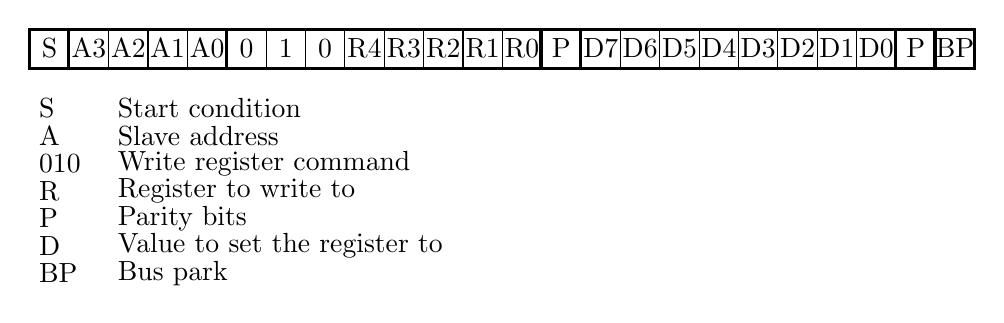
\begin{tikzpicture}[scale=0.5]
        \tikzstyle{bit} = [minimum height=5mm, minimum width=5mm, inner sep=0pt, draw];
        \foreach \i/\j in {
            0/S, 
            1/A3, 2/A2, 3/A1, 4/A0,
            5/0, 6/1, 7/0, 8/R4, 9/R3, 10/R2, 11/R1, 12/R0, 13/P,
            14/D7, 15/D6, 16/D5, 17/D4, 18/D3, 19/D2, 20/D1, 21/D0, 22/P,
            23/BP
        } {
            \node [bit,anchor=south west] at (\i,0) {\j};
        };

        \draw[very thick] (0,0) rectangle (1,1);
        \draw[very thick] (1,0) rectangle (5,1);
        \draw[very thick] (5,0) rectangle (13,1);
        \draw[very thick] (13,0) rectangle (14,1);
        \draw[very thick] (14,0) rectangle (22,1);
        \draw[very thick] (22,0) rectangle (23,1);
        \draw[very thick] (23,0) rectangle (24,1);

        \tikzstyle{T} = [anchor=west];
        \begin{scope}[yshift=-10mm, yscale=0.7]
            \foreach \i/\j/\l in {
                0/S/Start condition,
                1/A/Slave address,
                2/010/Write register command,
                3/R/Register to write to,
                4/P/Parity bits,
                5/D/Value to set the register to,
                6/BP/Bus park
            } {
                \node[T] at (0,-\i) {\j};
                \node[T] at (2,-\i) {\l};
            };
        \end{scope}
    \end{tikzpicture}
    \caption{RFFE command for writing to a register.}
    \label{fig:rffe_write_register}
\end{figure}
The RFFE command used for writing to a register is shown in Figure~\ref{fig:rffe_write_register}. The sequence is clocked out serially. A one bit is observed when the SCLK line goes high while the SDATA line is high and a zero bit is observed when the SCLK line goes high while the SDATA line is low. The start, parity, and bus park condition are described as follows:
\begin{description}
    \item[Start] SDATA pulses high while the SCLK line is kept low.
    \item[Parity] The parity is low if the number of ones in the preceding byte is odd. The parity is high if the number of ones in the preceding byte is even.
    \item[Bus park] SCLK is pulsed while SDATA is kept low (i.e.\ a zero is clocked out).
\end{description}
An example of and RFFE Write Register command is shown in Figure~\ref{fig:rffe_example}, where \texttt{0x00} is written to register 1 of the slave with address \texttt{0b0111}. This is the RFFE output when sending the string \texttt{"Ax0"} to the microcontroller, according to Table~\ref{tab:rffe_commands}.

\begin{figure}[htbp]
    \centering
    \includegraphics{img/optical_rffe/avr_rffe_reg1_0x00}
    \caption{Example of an RFFE command from the microcontroller.}
    \label{fig:rffe_example}
\end{figure}

\subsection{Level Shifting and WS1040 Interface}
The final part of the circuit is the interface towards the tuner. The microcontroller outputs signals between \SI{0}{V} and \SI{3.3}{V} which is not compatible with the tuner. Therefore, a level shifter is inserted, translating the \SI{3.3}{V} to \SI{1.8}{V}. The \SI{1.8}{V} is generated by a low-dropout voltage regulator.

\subsection{Testing}
An antenna board with tuner has been measured on a VNA and in the Satimo chamber, with and without the RFFE adaptor board to check if the $S$-parameters or total efficiency changes with the adaptor board present. The $S$-parameters and total efficiency, shown in Figure~\ref{fig:rffe_test_results}, shows no significant change when adding the RFFE adaptor board. The difference in the $S$-parameters may be because of slight bending due to handling of the antennas as the measurements were not done on the same day. The efficiency measurements were done the same day and shows no significant change. Another $S$-parameter measurement is shown in Figure~\ref{fig:rffe_test_results2} of another antenna. Here, the measurements are done in direct succession of each other and the $S$-parameters shows only \emph{very} little difference.

From the measurements just described, it has been verified that using the RFFE board with a fiber optic cable attached causes no significant change in $S$-parameters or total efficiency. Therefore, the board can be used for automating tests on a VNA and in the Satimo chamber.

\begin{figure}[htbp]
    \centering
    \begin{subfigure}[t]{0.49\linewidth}
        \includegraphics{img/optical_rffe/compare_sparams}
        \caption{$S$-parameters.} 
    \end{subfigure}
    \hfill
    \begin{subfigure}[t]{0.49\linewidth}
        \includegraphics{img/optical_rffe/compare_efficiency}
        \caption{Total efficiency.} 
    \end{subfigure}
    \caption{Comparison of the tuner PCB with and without the RFFE adaptor PCB.}
    \label{fig:rffe_test_results}
\end{figure}

\begin{figure}[htbp]
    \centering
    \includegraphics{img/optical_rffe/compare_sparams2}
    \caption{Comparison of $S$-parameters of the tuner PCB with and without RFFE adaptor PCB. }
    \label{fig:rffe_test_results2}
\end{figure}

\section{VNA Automatic Test}
\label{sec:vna_python}
In order to faster do sweep-measurements on the built prototypes, the VNA measurements have been automated and combined with the optical RFFE adapter. It is possible to control the VNA using GPIB (General Purpose Interface Bus), VISA protocol (Virtual Instrument Software Architecture), and SCPI (Standard Commands for Programmable Instruments). This has been implemented in Python and is specifically for a Rohde \& Schwarz ZVB 8 VNA, which is documented in this appendix. The library can be downloaded at \url{http://github.com/16gr1051}.

\subsection{National Instruments GPIB-USB-B Adapter}
A NI GPIB USB adapter is used for the communication between the PC and the VNA. For this to work in Linux, a few modifications are needed. First, the ni-gpib kernel module has to be loaded using \verb|modprobe ni_usb_gpib|. Next, a firmware update is needed, which has to be loaded every time. To ease pain, a small script has been made that does this step:
\begin{lstlisting}
#!/bin/bash
#Firmware files: http://linux-gpib.sourceforge.net/firmware/
usbDev="$(lsusb | grep "3923:702b National" | sed 's/://' | awk '{print $2 "/" $4}')"

if [ -z "$usbDev" ]; then
   echo "NIgpib device not found"
else
   modprobe ni_usb_gpib
   fxload -D /dev/bus/usb/$usbDev -I %/lib/firmware/ni_usb_gpib/niusbb_firmware.hex -s %/lib/firmware/ni_usb_gpib/niusbb_loader.hex    
fi
\end{lstlisting}

\subsection{Python Library}
The procedure for installing this library is shown in Section~\ref{sec:pythoninstall}.

The Python library is based around Pyvisa, which handles the VISA and SCPI protocol part and the communication with the USB GPIB adapter. The Rohde \& Schwarz ZVB 8 operating manual~\cite{RhodeSmanual} contains a chapter with all SCPI commands used. The library handles the setup of the VNA, which includes the correct frequency range, labels, and number of samples. Besides the setup function, it also contains a save function which changes the number of samples and exports the data formatted as a \verb|s2p| file. Below is an example of initializing the VNA and saving a sweep. 
\begin{lstlisting}
from vnalib import VNA
# Connect to VNA and initialize
myVNA = VNA("GPIB0::20::INSTR", "D:\\vna_measurement\\")
myVNA.initSettings()
# Save s2p file
myVNA.save("myfile")
\end{lstlisting}
 
\subsubsection{Combining with the Optical RFFE Adapter}
To fully automate the sweeping process, the code has been combined with the optical RFFE adapter board. The adapter board requires a serial command, which is sent using the pyserial library. The combined program is then able to sweep through every capacitor value and save a file for every measurement. This program is listed below. 
\begin{lstlisting}
from vnalib import VNA
import time
import serial
serial_port = "/dev/ttyUSB0"
basename = "triag"

# Connect to VNA
myVNA = VNA("GPIB0::20::INSTR", "D:\\vna_measurements\\")
myVNA.initSettings()
input("Perform manual calibration and press Enter...")

# Start serial port
ser = serial.Serial(serial_port)
ser.flushInput()
ser.flushOutput()

# Only slave address A = 0x7 is used
ser.write(b"Ax0Ay0Az0At0")

# Start sweep
for x in [
        ["0_0_0_0", b"Ax0Ay0Az0At0"],
        ["2_0_0_0", b"Ax2Ay0Az0At0"],
        ["4_0_0_0", b"Ax4Ay0Az0At0"],
        ...
        ["f_f_f_f", b"AxfAyfAzfAtf"],
        ]:
    fname,cmd = x
    fname = basename + "_" + fname
    ser.write(cmd)
    input("")
    myVNA.save(fname)
    print("Saved file")
\end{lstlisting}

\section{Satimo Automatic Test}
\label{sec:satimo_python}
The efficiency measurements are in general the most time consuming, and automating this process saves a lot of time. Unfortunately there is no public API or common interface to control the Satimo chamber. Therefor the only way to control the chamber is to automate the GUI (Graphical User Interface), which is done in Python.

\subsection{Python Library}
The procedure for installing this library is shown in Section~\ref{sec:pythoninstall}.

The Python library is based around another library called pywinauto, which is for Windows GUI Automation. Basically it sends ``click'' and ``keystroke'' events to specific buttons and input fields programmatically. Another tool called SWAPY was used to find button and input field IDs. 

Currently the created library only supports Satimo Passive measurements, and it is able to initiate a frequency sweep in a given frequency range and number of samples. The library detects when a sweep is done, and automatically exports the data in a \verb|TRX| file. The library also makes it easier to calibrate Satimo, such that the user only has to change the antenna and press \verb|Enter|, for each calibration antenna. Below is an example of calibrating, starting a sweep and exporting the data.  

\begin{lstlisting}
import satimopm
satimopm.calib()
satimopm.satimoSPM(startFreq, endFreq, samples, filename)
print("Sweep done")
\end{lstlisting}
 
\subsubsection{Combining with the Optical RFFE adapter}
As with the VNA library, we can combine the Satimo automation code with the optical RFFE adapter board. The adapter board, requires a serial command, which is done using the pyserial library. The combined program is then able to sweep through every capacitor value and save a file for every measurement. This program is listed below. 

\begin{lstlisting}
import satimopm
import serial

basename = "triag_top_vert"
serial_port = "/dev/ttyUSB0"

# Start serial port
ser = serial.Serial(serial_port)
ser.flushInput()
ser.flushOutput()

# Only slave address A = 0x7 is used
ser.write(b"Ax0Ay0Az0At0")

# Start sweep
for x in [
        ["0_0_0_0", b"Ax0Ay0Az0At0"],
        ["2_0_0_0", b"Ax2Ay0Az0At0"],
        ["4_0_0_0", b"Ax4Ay0Az0At0"],
        ...
        ["f_f_f_f", b"AxfAyfAzfAtf"],
        ]:
    fname,cmd = x
    fname = basename + "_" + fname
    ser.write(cmd)
    satimopm.measure(fname)

ser.close()
\end{lstlisting}

Here the \verb|measure| is a function, which contains a collection of calls to the more basic \verb|satimopm.satimoSPM|.







\chapter{Post Processing}
\label{cha:postproc}

In this chapter, the libraries for post processing data from CST and Satimo will be described. The libraries are written in Python. By the end of the chapter, usage examples will be given.

\section{Data Format}
The trx files, from Satimo Passive Measurement, contain data formatted in four columns:
\begin{enumerate}
    \item Horizontal polarization, real part.
    \item Horizontal polarization, imaginary part.
    \item Vertical polarization, real part.
    \item Vertical polarization, imaginary part.
\end{enumerate}
Each column contains 
\begin{equation}
    n_r =  n_f \times n_a \times n_e
\end{equation}
where
\begin{where}
\item[$n_r$] Total number of rows per column.
\item[$n_f$] Number of different frequencies in the measurement.
\item[$n_a$] Number of azimuth coordinates (usually 8).
\item[$n_e$] Number of elevation coordinates (usually 15).
\end{where}
The first $n_a \times n_e$ rows are for the first frequency and the next $n_a \times n_e$ rows are for the second frequency. Within this, the first $n_e$ rows are for the first azimuth angle and so on.

To get a better overview, the basic format for the following libraries is a $\theta \times \phi$-matrix like the following:
\begin{equation}
    M = \begin{bmatrix}
        m_{1,1} & m_{1,2} & \dots & m_{1,n} \\
        m_{2,1} & m_{2,2} & \dots & m_{2,n} \\
        \vdots & \vdots & & \vdots \\
        m_{m,1} & m_{m,2} & \dots & m_{m,n}
    \end{bmatrix}
\end{equation}
The data is rearranged to have $\phi$ go from \ang{0} to \ang{360} and $\theta$ from \ang{0} to \ang{180} as shown in Table~\ref{tab:matrixformat}.

\begin{table}[htbp]
    \centering
    \begin{tabular}{|l|c|c|}
        \hline
        Elements & $\theta$ & $\phi$ \\
        \hline
        $m_{1,1}$ & \ang{0} & \ang{0} \\
        $m_{1,n}$ & \ang{0} & $\ang{360}$ \\
        $m_{m,1}$ & \ang{180}$^{\dagger}$ & \ang{0} \\
        \hline
    \end{tabular}
    \caption{Format of $\theta\times\phi$-matrix. $^{\dagger}$For Satimo measurements, this is $180-22.5=\ang{157.5}$ because of the blind spot in the bottom.}
    \label{tab:matrixformat}
\end{table}

\section{Satimo StarLab Anechoic Chamber}

\begin{aautop}
    The farfield measurements for this project will be carried out in a StarLab anechoic chamber by Satimo. In this section, the basic principles of doing measurements in this chamber will be described.
\end{aautop}

\begin{figure}[htbp]
    \centering
    \begin{subfigure}[t]{0.49\linewidth} 
        \centering
        \includegraphics{img/analysis/satimo}
        \caption{Satimo StarLab. Modified from \cite{satimo}.}
        \label{fig:starlabchamber}
    \end{subfigure}
    \hfill
    \begin{subfigure}[t]{0.49\linewidth}
        \centering
        \includegraphics{img/analysis/satimoflow}
        \caption{Flow of a typical passive Satimo measurement.}
        \label{fig:satimoflow}
    \end{subfigure}
    \caption{Satimo StarLab passive measurement procedure.}
\end{figure}

The Satimo chamber is shown in Figure~\ref{fig:starlabchamber}. It consists of fifteen dual-polarized probes arranged in a circle with \ang{22.5} between each. The probes are located in a circle of absorbing cones and the whole machine is placed in a shielded room.

% Passive measurements: Power -> Antenna -> Probes
% What is measured?
The measurements used in this project are passive measurements. This means that the power is supplied from outside the chamber to the Device Under Test (DUT), which then radiates. The source is a user defined frequency sweep. For each frequency, the real and imaginary field at each probe for each polarization is sampled and recorded to a PC. After all frequencies for all probes have been recorded, the bed of the DUT turns, e.g.\ \ang{22.5}, and the procedure repeats. The flow is shown in Figure~\ref{fig:satimoflow}. The output is stored in a \texttt{trx} file in the order described by the flow chart. The post processing of the \texttt{trx} files is described thoroughly in Appendix~\ref{cha:postproc}.

% What we will use: Efficiency and correlation
% Calibration: Reference gain and efficiency
The measurements used for this report will mainly be used to compute the total efficiency of the DUT.
The efficiency can be computed by first calibrating the measurements by measuring a reference antenna with a known efficiency. The procedure for this is described in Section~\ref{sec:mimoant}.

%% Sources of error
The Satimo chamber is quite a complex system, and there are many sources of error. However, some of them are the same as with the VNA, which was described in Section~\ref{vna:errorSource}. Furthermore, there can be current flowing on the cable, bad connections, misaligned probes and inaccuracy in the motor rotations. 

\begin{aautail}
In this section, the Satimo StarLab chamber has been described. Based on this, the farfields can be measured of the antennas. By measuring reference antennas, the total efficiency can be computed. 
This section concludes the problem analysis, and the fundamental theorems and theories behind this project have been described. This leads to the final problem statement, which will briefly sum up the problem investigated throughout the rest of the report.
\end{aautail}

\section{CST Library}
In order to compare measurements and simulations, a library for processing CST simulations has been created. This makes it possible to import farfields, etc, from CST and convert them to the common data format described above. Once the data is in this format, the same functions can be used on measurements and simulations (e.g.\ computing envelope correlation coefficient).

\subsection{Function Documentation}
\subsubsection{col2mat(column, nx=360, ny=181)}
Convert a CST-exported column to a matrix with phi the 
x-axis and theta on the y-axis.

\begin{lstlisting}[numbers=none, frame=none, xleftmargin=0em, language=, basicstyle=\footnotesize\ttfamily]
- column: Column from a Satimo export.
- nx: Number of columns in the output (phi in the input).
- ny: Number of rows in the output (theta in the input).

Return:
Matrix with phi on the x-axis and theta on the y-axis.
\end{lstlisting}

\subsubsection{loadff(f)}
Load a CST exported file to two (theta x phi) matrices -- one for theta and
one for phi polarization.

\begin{lstlisting}[numbers=none, frame=none, xleftmargin=0em, language=, basicstyle=\footnotesize\ttfamily]
- f: File to load.

Return:
[T,P] where T and P are each a (theta x phi) matrix.
\end{lstlisting}



\section{3D Library}

The 3D library is created for plotting $\theta \times \phi$-matrices as well as computing the farfield envelope correlation coefficient between two farfields.

\subsection{Function Documentation}
\subsubsection{ecc(Eth1, Eth2, Eph1, Eph2)}
Compute the envelope correlation coefficient between two farfields. The
farfields are split into $\theta$ and $\phi$ part. Each part is a matrix with
$\theta$ on one axis and $\phi$ on the other.

\begin{lstlisting}[numbers=none, frame=none, xleftmargin=0em, language=, basicstyle=\footnotesize\ttfamily]
- Eth1: E-field, theta part, antenna 1
- Eth2: E-field, theta part, antenna 2
- Eph1: E-field, phi part, antenna 1
- Eph1: E-field, phi part, antenna 2

Return:
Envelope Correlation Coefficient (scalar)

Note:
https://mns.ifn.et.tu-dresden.de/Lists/nPublications/Attachments/612/Wang_Q_WSA_10.pdf
\end{lstlisting}

\subsubsection{intsphere(r, theta, phi)}
Do a spherical integral of a $(\theta \times \phi)$ matrix.

\begin{lstlisting}[numbers=none, frame=none, xleftmargin=0em, language=, basicstyle=\footnotesize\ttfamily]
- r: Matrix to integrate (x-axis=phi, y-axis=theta).
- phi: Phi axis values.
- theta: Theta axis values.

Return:
Scalar result of the integration.
\end{lstlisting}

\subsubsection{plot3d(r, stride=1, th\_lim=(0, 180), ph\_lim=(0, 360))}
Plot a matrix, $(\theta \times \phi)$, in 3D space.

\begin{lstlisting}[numbers=none, frame=none, xleftmargin=0em, language=, basicstyle=\footnotesize\ttfamily]
- r: Matrix to plot.
- stride: Resolution of the output. 1=detailed+slow, 10=rough+fast.
- th_lim: Upper and lower theta limits (degrees).
- ph_lim: Upper and lower phi limits (degrees).
\end{lstlisting}

\subsubsection{plotflat(r, th\_lim=(0,180), ph\_lim=(0,360), cmap="jet")}
Plot a farfield-matrix as a color-map. Remember that \ang{0} is the bottom of
the plot in spherical coordinates.

\begin{lstlisting}[numbers=none, frame=none, xleftmargin=0em, language=, basicstyle=\footnotesize\ttfamily]
- r: Matrix to plot (theta x phi).
- th_lim: Minimum and maximum theta/y-axis value (degrees).
- ph_lim: Minimum and maximum phi/x-axis value (degrees).
- cmap: Color map to use.
\end{lstlisting}



\section{Plotting Library: aauplot}
\label{sec:aauplotlib}

This library contains plotting functions to make plots consistent throughout the report. The plots contain markers for the LTE frequency bands to clearly signify what is in-band and out-of-band.

\subsection{Function Documentation}
\subsubsection{correlation(f, ecc, c="-", label="")}
Plot correlation

\begin{lstlisting}[numbers=none, frame=none, xleftmargin=0em, language=, basicstyle=\footnotesize\ttfamily]
- f: Frequency axis.
- ecc: Envelope correlation coefficient.
- c: Color/linetype string (e.g. '--b' for dashed blue).
- label: Label for the graph's legend.
\end{lstlisting}

\subsubsection{efficiency(f, e, c="-", label="")}
Plot an efficiency graph.

\begin{lstlisting}[numbers=none, frame=none, xleftmargin=0em, language=, basicstyle=\footnotesize\ttfamily]
- f: Frequency axis.
- e: Efficiency (. or dB).
- c: Color/linetype string (e.g. '--b' for dashed blue).
- label: Label for the graph's legend.
\end{lstlisting}

\subsubsection{end\_correlation(loc=1, fontsize=8)}
Finish the correlation plot with legend, etc.

\begin{lstlisting}[numbers=none, frame=none, xleftmargin=0em, language=, basicstyle=\footnotesize\ttfamily]
- loc: Location of the legend (like matplotlib.pyplot.legend())
- fontsize: Font size for the legend.
\end{lstlisting}

\subsubsection{end\_efficiency(**kwargs)}
Finish the efficiency plot with legend, etc.

\begin{lstlisting}[numbers=none, frame=none, xleftmargin=0em, language=, basicstyle=\footnotesize\ttfamily]
- kwargs: Arguments passed on to matplotlib.pyplot.legend()
\end{lstlisting}

\subsubsection{end\_sar(**kwargs)}
Finish the SAR plot with legend, etc.

\begin{lstlisting}[numbers=none, frame=none, xleftmargin=0em, language=, basicstyle=\footnotesize\ttfamily]
- kwargs: Arguments passed on to matplotlib.pyplot.legend()
\end{lstlisting}

\subsubsection{end\_sparam(**kwargs)}
Finish the $S$-parameter plot with legend, etc.

\begin{lstlisting}[numbers=none, frame=none, xleftmargin=0em, language=, basicstyle=\footnotesize\ttfamily]
- kwargs: Parameters passed onto matplotlib.pyplot.legend().
\end{lstlisting}

\subsubsection{figure(*args, **kwargs)}
Set up a figure of the correct dimensions and the correct font for the
report.

\begin{lstlisting}[numbers=none, frame=none, xleftmargin=0em, language=, basicstyle=\footnotesize\ttfamily]
- args: Positional arguments for matplotlib.pyplot.figure()
- kwargs: All arguments are passed onto the matplotlib.pyplot.figure()
        function.
\end{lstlisting}

\subsubsection{freqscale(f)}
Scale to get frequency axis to MHz

\begin{lstlisting}[numbers=none, frame=none, xleftmargin=0em, language=, basicstyle=\footnotesize\ttfamily]
- f: Frequency axis.
\end{lstlisting}

\subsubsection{sar(f, sar, c="-", label="")}
Plot a SAR graph.

\begin{lstlisting}[numbers=none, frame=none, xleftmargin=0em, language=, basicstyle=\footnotesize\ttfamily]
- f: Frequency axis.
- e: Efficiency (. or dB).
- c: Color/linetype string (e.g. '--b' for dashed blue).
- label: Label for the graph's legend.
\end{lstlisting}

\subsubsection{sparam(f, s, c="-", label="")}
Plot an $S$-parameter.

\begin{lstlisting}[numbers=none, frame=none, xleftmargin=0em, language=, basicstyle=\footnotesize\ttfamily]
- f: Frequency axis for the plot.
- s: S-parameter (abs-value in dB) to plot.
- c: Color/linetype string (e.g. '--b' for dashed blue).
- label: Label for the legend
\end{lstlisting}

\subsubsection{to\_db(x)}
Convert/preserve data in dB

\begin{lstlisting}[numbers=none, frame=none, xleftmargin=0em, language=, basicstyle=\footnotesize\ttfamily]
- x: Data to convert (e.g. efficiency).

Return:
Data in dB.
\end{lstlisting}



\section{Examples}

\subsection{Extract Efficiency from Satimo}
In the following example, the efficiency of an antenna is extracted. In order to do this, calibration measurements must be added to the \texttt{calfiles} list. The \texttt{reffiles} list contains reference data of the antennas used for calibration. \emph{Note, that the files from these two lists must be written in ascending order, i.e.\ lowest frequency first}. In this example, the file \texttt{antenna\_meas.trx} is the antenna from which the efficiency is extracted. The output is saved to the file shown in Figure~\ref{fig:pp_example1}.

\lstinputlisting[caption={Extracting efficiency from Satimo.}, label=lst:ex1]{sec/post_processing/examples/example1.py}

\begin{figure}[htbp]
    \centering
    \includegraphics[scale=0.5]{sec/post_processing/examples/ex1_efficiency.pdf}
    \caption{Output from Listing~\ref{lst:ex1}.}
    \label{fig:pp_example1}
\end{figure}


\subsection{Plot 3D Farfield}
The (rough) farfield directly exported from Satimo's 15 probes can be plotted in 3D as shown below. The result is shown in Figure~\ref{fig:pp_example2}. A similar plot -- a 2D color plot -- is also plotted.

\lstinputlisting[caption={Plot 3D Farfield.}, label=lst:ex2]{sec/post_processing/examples/example2.py}

\begin{figure}[htbp]
    \centering
    \begin{subfigure}{0.49\linewidth}
        \centering
        \includegraphics[scale=0.5]{sec/post_processing/examples/ex2_3dfarfield.pdf}
        \caption{3D.}
    \end{subfigure}
    \hfill
    \begin{subfigure}{0.49\linewidth}
        \centering
        \includegraphics[scale=0.5]{sec/post_processing/examples/ex2_2dfarfield.pdf}
        \caption{2D.}
    \end{subfigure}
    \caption{Output from Listing~\ref{lst:ex2}.}
    \label{fig:pp_example2}
\end{figure}

\subsection{Import a Farfield from CST}
The following example will import and plot a farfield from CST. The farfield should be exported under the Post Processing tab. The output is shown in Figure~\ref{fig:pp_example3}.

\lstinputlisting[caption={Import a Farfield from CST.}, label=lst:ex3]{sec/post_processing/examples/example3.py}


\begin{figure}[htbp]
    \centering
    \begin{subfigure}{0.49\linewidth}
        \centering
        \includegraphics[scale=0.5]{sec/post_processing/examples/ex3_3dfarfield.pdf}
        \caption{3D.}
    \end{subfigure}
    \hfill
    \begin{subfigure}{0.49\linewidth}
        \centering
        \includegraphics[scale=0.5]{sec/post_processing/examples/ex3_2dfarfield.pdf}
        \caption{2D.}
    \end{subfigure}
    \caption{Output from Listing~\ref{lst:ex3}.}
    \label{fig:pp_example3}
\end{figure}

\subsection{Export Efficiency for Further Analysis}
Using python and numpy, analysis and comparison can be done just as easily as in MATLAB. However, if one is more familiar with MATLAB or need the data for other software, it is advantageous to export the data. Here is a simple example of exporting the efficiency as a data file.

\lstinputlisting[caption={Export efficiency for further analysis.}, label=lst:ex4]{sec/post_processing/examples/example4.py}

The output is a tab-separated file (\texttt{ex4\_efficiency.txt}) which can easily be imported into MATLAB or similar software.

\subsection{Plots for IEEEtran Articles}
It is often desirable to export graphs in a format that is compliant with the text used articles. In the standard IEEEtran format, a \emph{Times} font is used. For figures, the default font size is 8\,pt. The column width is \SI{3.5}{inches}. In the example, the figure size is set to $\SI{3.5}{inches}\times \SI{3}{inches}$.

Note that math symbols can easily be used in figure text (e.g.\ labels) in the same way as symbols are written in \LaTeX, e.g.\ ``\verb|$\theta$ in degrees|'' becomes ``$\theta$ in degrees''.

The result is shown in Figure~\ref{fig:pp_example5}.

\lstinputlisting[caption={Plots for IEEEtran articles.}, label=lst:ex5]{sec/post_processing/examples/example5.py}

\begin{figure}[htbp]
    \centering
    \includegraphics{sec/post_processing/examples/ex5_efficiency.pdf}
    \caption{Output from Listing~\ref{lst:ex5}.}
    \label{fig:pp_example5}
\end{figure}



% \section{User Effect - Simulation}


\subsubsection{Hand Simulation}
\begin{itemize}
\item 1 hand - Data mode
\begin{itemize}
\item Align antenna design with upper spacer.
\item Move the antenna design down until touching the lower spacer
\item If the antenna is longer than the lenght from the lower to the upper spacer, the antenna design exceeds the upper spacer.
\end{itemize}
\item 1 hand - talk mode (SAR measurement)
\begin{itemize}
\item Antenna design is aligned with the Antenna design in the ``SAR
\item 
\end{itemize}
\end{itemize}

\subsubsection{Head Simulation}
\begin{itemize}
\item SAR measurement
\begin{itemize}
\item Antenna design is aligned with the Antenna design in the ``SAR
\item 
\item 
\end{itemize}
\end{itemize}


% Back matter %%%%%%%%%%%%%%%%%%%%%%%%%%%%%%%%%%%%%%%%%%%%%%%%%%%%%%%%%%%%%%%%%%

\listoffixmes
\bibliographystyle{ieeetr}
\bibliography{bib/sources}
\addcontentsline{toc}{chapter}{Bibliography}

\end{document}
